\documentclass[11pt,a4paper]{article}

\usepackage[utf8]{inputenc}
\usepackage[T1]{fontenc}
\usepackage{geometry}
\geometry{top=2.2cm,bottom=2.2cm,left=2.3cm,right=2.3cm}
\usepackage{graphicx}
\graphicspath{{figures/}}
\usepackage{booktabs}
\usepackage{tabularx}
\usepackage{xltabular}
\usepackage{longtable}
\usepackage{array}
\usepackage{ragged2e}
\usepackage{float}
\usepackage{subcaption}
\usepackage{caption}
\usepackage{amsmath}
\usepackage{enumitem}
\usepackage{setspace}
\usepackage{microtype}
\usepackage[hypertexnames=false]{hyperref}
\usepackage{xcolor}
\usepackage[section]{placeins}
\usepackage{xurl}
\usepackage{lmodern}
\setlength{\emergencystretch}{2em}

\setstretch{1.06}
\setlength{\parskip}{0.35em}
\setlength{\parindent}{0pt}
\captionsetup{justification=centering,font=small}
\hypersetup{
    colorlinks=true,
    linkcolor=black,
    citecolor=black,
    urlcolor=black
}
\setlist[itemize]{nosep,leftmargin=1.5em}
\setlist[enumerate]{nosep,leftmargin=1.7em}

\newcommand{\code}[1]{\texttt{#1}}

\title{
    \vspace{1.0cm}
    \normalsize UNIVERSITY OF KWAZULU-NATAL \\
    COMP721: Machine Learning \\
    \large \textbf{Semester Project - Phase 3 Final Technical Report} \\
    \normalsize Cardiovascular Disease Risk Prediction Using Classical Machine Learning,
    Ensemble Learning, and Explainable Artificial Intelligence
}

\author{
    \small
    \textbf{Group 3} \\
    Lokadi Naicker \\
    Arjun Ramphal \\
    Keolin Naicker \\
    Darian Robert
}

\date{\small Submission Date: 28 October 2026}

\newif\ifreviewmode
\reviewmodefalse
\let\originalincludegraphics\includegraphics
\renewcommand{\includegraphics}[2][]{%
  \ifreviewmode
    \IfFileExists{figures/#2}{\originalincludegraphics[#1]{#2}}{%
      \fbox{\parbox[c][0.24\textheight][c]{0.88\linewidth}{\centering
      Figure unavailable in the uploaded materials\\[0.5em]
      \texttt{\detokenize{#2}}}}}%
  \else\originalincludegraphics[#1]{#2}\fi}

\begin{document}
\begin{titlepage}
\maketitle
\thispagestyle{empty}
\pagenumbering{arabic}
\begin{abstract}
Cardiovascular disease (CVD) remains a major global health burden, motivating reliable and interpretable methods for classifying patients using routinely collected demographic, physiological, and lifestyle information. This project developed an end-to-end classical machine learning pipeline using the 70,000-record Cardiovascular Disease dataset. After removing duplicates, correcting or removing inconsistent observations, and treating outliers based on plausibility, 68,517 records remained. Eleven engineered variables were added, including Body Mass Index, pulse pressure, mean arterial pressure, hypertension stage, composite risk indicators, and an age--cholesterol interaction. Recursive Feature Elimination selected five predictors -- \code{ap\_hi}, \code{age\_cholesterol\_interaction}, \code{age\_years}, \code{bmi}, and \code{map} -- while approximately preserving the mean cross-validation accuracy of the complete 22-feature representation; both results rounded to 72.82\%.

A Decision Tree and Support Vector Machine (SVM) were tuned over four prescribed configurations using five-fold stratified cross-validation on the training partition only. A Soft Voting ensemble and a Stacking candidate were then compared using the same aligned folds without using the held-out test set for ensemble selection. Soft Voting achieved the higher mean validation accuracy (73.27\% versus 73.07\%) and was selected as the final ensemble. On the held-out test set, the SVM obtained the highest accuracy (73.47\%), while Soft Voting obtained 73.45\% accuracy and the strongest F1-score (71.81\%), ROC-AUC (0.7935), and Average Precision (0.7756). SHAP analysis consistently ranked systolic blood pressure as the most influential predictor, followed by the age--cholesterol interaction. Paired five-fold testing showed that Soft Voting significantly outperformed the Decision Tree ($p=0.0040$), but not the SVM ($p=0.0864$). The results therefore support a modest ensemble benefit, but not a statistically demonstrated advantage over the strongest individual classifier.
\end{abstract}

\end{titlepage}
\clearpage
\section{Introduction}

\subsection{Background and Motivation}

Cardiovascular disease (CVD) accounts for approximately 32\% of global deaths \cite{who2025}, making early identification of patients with adverse cardiovascular profiles an important healthcare objective. Machine learning is suitable for this task because it can model interactions among demographic, physiological, and lifestyle variables that may be difficult to express using simple univariate rules. Ensemble methods are particularly relevant because they combine complementary classifiers and can improve generalisation when the component models make different errors \cite{patra2023,tiwari2022}. Explainable artificial intelligence (XAI) techniques such as SHAP can further improve transparency by identifying the features that contribute most strongly to individual predictions \cite{shah2025}.

\subsection{Problem Statement and Scope}

The project title uses the term \emph{risk prediction}; however, the available dataset contains a binary \code{cardio} label indicating observed CVD absence or presence rather than prospective future cardiovascular events. The implemented system should therefore be interpreted as a CVD status classifier based on the observed variables, not as a longitudinal clinical risk score.

The project addresses three linked questions. First, can careful preprocessing, feature engineering, and feature selection produce a compact representation without reducing predictive performance? Second, does combining a tuned Decision Tree and SVM into an ensemble provide a meaningful and statistically significant improvement over the individual classifiers? Third, can SHAP explanations identify clinically plausible drivers of the model outputs and provide useful local explanations for individual patients?

\subsection{Aim and Objectives}

The overall aim was to evaluate whether an interpretable ensemble of classical classifiers improves CVD status classification over its individual components.

The specific objectives were to:
\begin{itemize}
    \item clean and preprocess the dataset while justifying duplicate handling, inconsistent-value treatment, encoding, scaling, and outlier decisions;
    \item perform exploratory data analysis to identify distributions, associations, class balance, and data-quality issues;
    \item engineer at least five new variables, including medically meaningful features supported by literature;
    \item compare original, engineered, and selected predictor subsets and justify the final feature representation;
    \item tune a Decision Tree and an SVM over four configurations each using five-fold cross-validation;
    \item construct an ensemble from the two tuned base models and determine whether Soft Voting or Stacking is the more appropriate final ensemble using training cross-validation only;
    \item evaluate the final models using accuracy, precision, recall, specificity, F1-score, ROC-AUC, Average Precision, MCC, and Cohen's Kappa;
    \item explain model behaviour globally and locally using SHAP; and
    \item statistically test whether the selected ensemble improves on the Decision Tree and SVM using paired five-fold scores.
\end{itemize}

\subsection{Report Organisation}

Section~2 reviews related work. Section~3 describes the methodology, and Section~4 records the experimental setup. Section~5 presents the results. Section~6 interprets the findings, limitations, and future work, before Section~7 concludes the report.

\section{Literature Review}


\subsection{Cardiovascular Classification and Ensemble Learning}
Cardiovascular prediction studies differ in their outcomes and populations. Patra et al. investigate ten-year coronary heart disease prediction using Framingham data, forward selection, and a two-step voting ensemble \cite{patra2023}. Their work motivates combining feature selection with heterogeneous learning, but its prospective outcome differs from the observed-status target studied here.

Tiwari et al. develop a stacked ensemble using a combined dataset drawn from Hungarian, Cleveland, Long Beach VA, Switzerland, and Statlog sources \cite{tiwari2022}. Their framework includes ExtraTrees, Random Forest, and XGBoost. It supports investigating multiple learners, although a result from that dataset cannot establish that a Decision Tree--SVM ensemble will improve on either component in the present experiment.

\subsection{Feature Engineering and Selection}
Clinical transformations can express relationships more directly than individual measurements: BMI relates weight to height, while pulse pressure and MAP summarise blood-pressure measurements \cite{whoObesity2025,sesso2000}. Such transformations add representations rather than new measurements. They can help a constrained learner, but may also introduce redundant predictors.

Theerthagiri and Vidya combine RFE with gradient boosting on the Kaggle cardiovascular dataset \cite{theerthagiri2022}. Their study reports favourable performance for the combined approach, motivating an empirical comparison of reduced and complete predictor sets. The present study instead uses a depth-limited Decision Tree as the RFE reference estimator and compares ANOVA, Mutual Information, and RFE under the same training-data protocol. Dritsas and Trigka provide further context for systematic comparison of data-driven cardiovascular models \cite{dritsas2023}.

\subsection{Explainability and Evaluation}
Shah et al. investigate hybrid ensemble learning together with explainable AI for cardiovascular prediction \cite{shah2025}. This motivates evaluating both predictive performance and feature-level explanations. SHAP attributes a model output to input features relative to a background distribution \cite{lundberg2017}; it explains the fitted prediction function rather than establishing a causal medical relationship.

Model selection also affects the credibility of reported performance. Cawley and Talbot discuss selection bias arising when evaluation is used to optimise a model \cite{cawley2010}. Accordingly, this study separates training-based selection from final testing and explicitly records where feature selection is fitted within folds and where a fixed representation is subsequently reused.

\subsection{Comparison and Position of the Present Study}
Table~\ref{tab:literature} compares the principal methodological connections. These are comparisons of research design; published accuracy values are not used as a leaderboard because outcomes, cleaning rules, models, and validation procedures differ.

{\small
\begin{xltabular}{\textwidth}{@{}p{2.7cm}XXX@{}}
\caption{Related studies and their relevance to the present experiment.}\label{tab:literature}\\
\toprule
\textbf{Study} & \textbf{Data / task} & \textbf{Approach / finding} & \textbf{Relevance and distinction}\\
\midrule\endfirsthead
\toprule\textbf{Study} & \textbf{Data / task} & \textbf{Approach / finding} & \textbf{Relevance and distinction}\\\midrule\endhead
\bottomrule\endlastfoot
Patra et al. \cite{patra2023} & Framingham; ten-year CHD risk. & Forward selection and two-step hybrid voting; compact predictive representation. & Motivates selection plus ensembling; outcome differs from observed CVD status.\\
Tiwari et al. \cite{tiwari2022} & Combined five-source heart-disease dataset. & Stacking with several tree-based learners; favourable classification reported. & Motivates ensemble comparison; different data and component models.\\
Theerthagiri and Vidya \cite{theerthagiri2022} & Kaggle cardiovascular dataset. & RFE with gradient boosting; favourable reported performance. & Closely related selection setting; different reference learner and evaluation procedure.\\
Shah et al. \cite{shah2025} & Cardiovascular prediction. & Hybrid ensemble with explainable AI. & Motivates transparent ensemble analysis; not a matched experimental baseline.\\
Dritsas and Trigka \cite{dritsas2023} & Cardiovascular risk-prediction study. & Comparison of data-driven ML models. & Context for systematic model comparison; this project fixes DT and SVM as required learners.\\
\end{xltabular}}

The contribution of this project is an integrated, reproducible comparison within the prescribed coursework setting: clinically motivated engineered features, training-based feature-subset selection, four configurations per individual model, aligned ensemble comparison, a final held-out evaluation, comparable SHAP explanations, and paired-fold statistical analysis. It evaluates whether the ensemble gain is supported by evidence rather than assuming that combining models guarantees improvement.

\section{Methodology}

\subsection{Dataset}

The raw dataset contains 70,000 patient records and 13 variables: one identifier, eleven predictors, and the binary target \code{cardio}. The original class distribution is effectively balanced, with 50.03\% Class~0 and 49.97\% Class~1 \cite{ulianova2019}. Table~\ref{tab:variables} summarises the variables.

{\small
\begin{xltabular}{\textwidth}{@{}llX@{}}
\caption{Raw dataset variables and descriptions.}
\label{tab:variables}\\
\toprule
\textbf{Variable} & \textbf{Category / type} & \textbf{Description}\\
\midrule
\endfirsthead
\toprule
\textbf{Variable} & \textbf{Category / type} & \textbf{Description}\\
\midrule
\endhead
\bottomrule
\endlastfoot
\code{id} & Objective, integer & Unique patient record identifier.\\
\code{age} & Objective, integer (days) & Patient age recorded in days.\\
\code{gender} & Objective, categorical & Raw coding: 1 = women, 2 = men.\\
\code{height} & Objective, integer (cm) & Patient height.\\
\code{weight} & Objective, float (kg) & Patient weight.\\
\code{ap\_hi} & Examination, integer (mmHg) & Systolic blood pressure.\\
\code{ap\_lo} & Examination, integer (mmHg) & Diastolic blood pressure.\\
\code{cholesterol} & Examination, ordinal & 1 = normal, 2 = above normal, 3 = well above normal.\\
\code{gluc} & Examination, ordinal & 1 = normal, 2 = above normal, 3 = well above normal.\\
\code{smoke} & Lifestyle, binary & Smoking indicator.\\
\code{alco} & Lifestyle, binary & Alcohol-intake indicator.\\
\code{active} & Lifestyle, binary & Physical-activity indicator.\\
\code{cardio} & Target, binary & CVD absent (0) or present (1).\\
\end{xltabular}
}

\subsection{Data Preprocessing}

Preprocessing was performed before feature engineering. Patient age was converted from days to years using
\[
\code{age\_years}=\frac{\code{age}}{365.25}.
\]
Duplicate detection excluded the unique \code{id} and the derived \code{age\_years} field but retained the original age value, so only records with identical underlying raw clinical information were treated as duplicates. The identifier was excluded from duplicate matching so that unique record IDs could not conceal repeated observations.

Missing-value counts were checked before deciding whether imputation was necessary. Negative systolic and/or diastolic blood-pressure values were converted to their absolute values under the explicit assumption that the negative sign represented a data-entry error. Because the original data source does not confirm the cause, this remains a preprocessing assumption. Rows with \code{ap\_lo} $\geq$ \code{ap\_hi} were then removed as internally inconsistent.

A purely IQR-based outlier rule was not used for deletion because it can remove clinically important high-risk observations. Instead, project-defined plausibility filters retained height $[125,215]$~cm, weight $[40,200]$~kg, systolic pressure $[70,250]$~mmHg, and diastolic pressure $[40,150]$~mmHg. These numerical limits were study-specific data-quality rules, not diagnostic thresholds prescribed by a clinical guideline. Blood-pressure guidance and obesity literature informed the general rationale for retaining clinically relevant hypertension and high-BMI observations \cite{whelton2018,whoObesity2025}, but do not independently validate these exact exclusion limits. Consequently, some residual measurement errors or unusual combinations may remain after filtering.

The identifier was dropped, and raw age was replaced with \code{age\_years}. Gender was recoded to 0 = women and 1 = men. Cholesterol and glucose retained their ordinal 1--3 coding, and the existing binary variables required no further encoding. Feature scaling was not applied globally; scaling required by the SVM was fitted inside training folds to prevent leakage.

\subsection{Exploratory Data Analysis Approach}

Distributions, descriptive statistics, class counts, boxplots, and Pearson correlations were examined to identify data-quality issues and relationships among the observed variables. Analyses distinguished statistical extremes from values excluded by the stated plausibility rules. The corresponding findings and figures are reported in Section~5. EDA in the submitted workflow used the cleaned dataset before splitting; feature-selection fitting and model tuning subsequently used the training partition only.

\subsection{Feature Engineering}

Eleven engineered variables were created from the cleaned predictors. The design aimed to introduce clinically interpretable transformations, threshold categories, interaction effects, and compact risk summaries while retaining a clear distinction between validated clinical definitions and project-defined heuristic features.

{\small
\begin{xltabular}{\textwidth}{@{}p{5.6cm}X@{}}
\caption{Engineered features and rationale.}
\label{tab:engineered}\\
\toprule
\textbf{Feature / computation} & \textbf{Rationale}\\
\midrule
\endfirsthead
\toprule
\textbf{Feature / computation} & \textbf{Rationale}\\
\midrule
\endhead
\bottomrule
\endlastfoot

\code{bmi}: weight / height$^2$ &
Body Mass Index calculated using weight in kilograms and height in metres:
$\code{weight}/(\code{height}/100)^2$. It represents an established
anthropometric measure associated with cardiometabolic risk
\cite{whoObesity2025}.\\

\code{pulse\_pressure}: \code{ap\_hi}-\code{ap\_lo} &
Captures the systolic--diastolic pressure difference, a cardiovascular
blood-pressure index investigated in the literature \cite{sesso2000}.\\

\code{map}: \code{ap\_lo} + \code{pulse\_pressure}/3 &
Approximates mean arterial pressure using the same blood-pressure
measurements; MAP has been investigated as a cardiovascular predictor
\cite{sesso2000}.\\

\code{htn\_stage}: 0--3 & ACC/AHA-inspired blood-pressure category using the more severe applicable systolic/diastolic stage \cite{whelton2018}.\\

\code{bmi\_category}: 0--3 & Underweight, normal, overweight, and obesity categories based on adult BMI thresholds \cite{whoObesity2025}.\\

\code{age\_category} & Project-defined groups $<40$, 40--49, 50--59, and $\geq60$ years.\\

\code{lifestyle\_risk}: smoke + alcohol + inactivity & Project-defined 0--3 heuristic summarising recognised modifiable risk factors \cite{who2025}.\\

\code{metabolic\_risk} & Project-defined composite using cholesterol severity, glucose severity, and obesity.\\

\code{cvd\_risk\_count} & Count of six adverse behavioural/physiological indicators; not a validated clinical score.\\

\code{metabolic\_risk\_flag} & Project-defined flag for multiple adverse metabolic characteristics; not a metabolic-syndrome diagnosis.\\

\code{age\_cholesterol\_interaction} & Product of age in years and cholesterol category to permit an age-dependent cholesterol effect.\\

\end{xltabular}
}

\subsubsection{Exact Definitions of Categories and Composite Features}

Let $S$ and $D$ denote systolic and diastolic pressure, respectively;
$A$ denotes age in years; $C$ and $G$ denote the original cholesterol and
glucose codes. The notation $\mathbf{1}[\cdot]$ equals one when its
condition is true and zero otherwise.

Hypertension category $H=\code{htn\_stage}$ was assigned in descending
order of severity:
\[
H=
\begin{cases}
3, & S\geq140 \text{ or } D\geq90,\\
2, & \text{otherwise, if } S\geq130 \text{ or } D\geq80,\\
1, & \text{otherwise, if } S\geq120,\\
0, & \text{otherwise}.
\end{cases}
\]
These categories encode ACC/AHA-inspired blood-pressure ranges
\cite{whelton2018}; a category derived from the available measurements
is not a confirmed clinical diagnosis.

BMI category $B=\code{bmi\_category}$ was coded as 0 for BMI $<18.5$,
1 for $18.5\leq\mathrm{BMI}<25$, 2 for
$25\leq\mathrm{BMI}<30$, and 3 for BMI $\geq30$.
Age category was coded as 0 for $A<40$, 1 for $40\leq A<50$,
2 for $50\leq A<60$, and 3 for $A\geq60$.

The composite features were calculated as follows:
\[
\code{lifestyle\_risk}
=
\code{smoke}+\code{alco}+(1-\code{active}),
\]
\[
\code{metabolic\_risk}
=
(C-1)+(G-1)+\mathbf{1}[B=3],
\]
\[
\begin{aligned}
\code{cvd\_risk\_count}
={}&\mathbf{1}[H\geq2]+\mathbf{1}[B\geq2]
+\mathbf{1}[\code{smoke}=1]\\
&+\mathbf{1}[C>1]+\mathbf{1}[G>1]
+\mathbf{1}[\code{active}=0],
\end{aligned}
\]
\[
\code{metabolic\_risk\_flag}
=
\mathbf{1}\!\left[
\mathbf{1}[B\geq2]+\mathbf{1}[H\geq2]+\mathbf{1}[C>1]\geq2
\right],
\]
and
\[
\code{age\_cholesterol\_interaction}=A\,C.
\]

The composite scores and interaction term are project-defined
transformations, not validated clinical risk instruments. In particular,
multiplying age by an ordinal cholesterol code does not represent a
measured cholesterol concentration. These transformations introduce no
new patient measurements; their intended benefit is to expose useful
thresholds, combinations, and interactions to the learning algorithms.
Whether they improve predictive performance must therefore be assessed
empirically.

\subsection{Feature Selection}

A single canonical 80/20 stratified split was created with \code{random\_state=42}: 54,813 training observations and 13,704 held-out test observations. The test set was not used during feature selection. Five-fold \code{StratifiedKFold} cross-validation with shuffling and \code{random\_state=42} was used consistently.

Three selection approaches were investigated:
\begin{itemize}
    \item ANOVA F-score using \code{SelectKBest};
    \item Mutual Information; and
    \item RFE using a Decision Tree with \code{max\_depth=5} as the reference estimator \cite{theerthagiri2022}.
\end{itemize}

For the feature-subset comparison, each selection method was fitted
inside the cross-validation training folds through a pipeline
\cite{cawley2010}. After selecting a method using the comparison, the chosen selector was fitted to the complete
54,813-record training partition to determine the final predictor identities.
The resulting fixed training and test subsets were saved for subsequent
model development.

Importantly, the later Decision Tree, SVM, and ensemble cross-validation
experiments reused this fixed five-feature representation rather than
refitting RFE inside each later fold. Those later scores therefore
evaluate classifiers conditional on the previously selected
representation; they are not fully nested estimates of the complete
feature-selection-and-classification procedure. The held-out test
partition was excluded from fitting the feature selectors.

\subsection{Model Development}

The two required individual models capture different structures in the tabular measurements \cite{pedregosa2011}.

\subsubsection{Decision Tree Classifier}
A Decision Tree recursively splits observations using feature thresholds that reduce class impurity. Its leaf nodes provide classifications and class-proportion probability estimates. This supports nonlinear threshold effects and interactions without requiring feature scaling. Maximum depth controls how many successive splits can be used; deeper trees can fit more specific patterns and may generalise less reliably. The model also provides Gini-based feature importance, which was examined separately from SHAP.

\subsubsection{Support Vector Machine}
An SVM learns a separating decision boundary by balancing a wide margin against classification errors. A kernel allows nonlinear similarity to be represented without explicitly constructing every transformed coordinate. Linear, polynomial, RBF, and sigmoid kernels were considered. Standardisation was included because SVM similarity and margin calculations depend on feature scale. An SVM provides a useful contrast to the axis-aligned thresholds of the tree; its probability estimates require an additional estimation step when used for soft voting.

\subsection{Hyperparameter Optimisation}

The required individual classifiers were a Decision Tree and SVM. Four configurations were evaluated for each:
\begin{itemize}
    \item Decision Tree: \code{max\_depth} $\in \{5,10,15,20\}$;
    \item SVM: linear, polynomial, RBF, and sigmoid kernels.
\end{itemize}
The Decision Tree configurations varied maximum depth to investigate
the trade-off between model complexity and generalisation. The four
SVM kernels provided linear and alternative nonlinear decision
boundaries. Configuration selection used mean five-fold training
accuracy, and the selected configurations were fitted to the complete
training partition.

The SVM used a \code{StandardScaler}--\code{SVC} pipeline, so scaling
parameters were fitted within each cross-validation training fold.
Other SVC settings retained their defaults, including $C=1$,
\code{gamma='scale'}, polynomial degree 3, and \code{coef0=0}.

Kernel comparison used \code{probability=False}. Probability estimation
was enabled for the final SVM and the fold-specific SVMs used in Soft
Voting. SVM classification accuracy was calculated from
\code{predict}, whereas ROC-AUC and Average Precision used
\code{predict\_proba}. Soft Voting used a fixed threshold of 0.5
on the averaged positive-class probabilities. No decision-threshold
search was performed.

\subsection{Cross-validation Strategy}

The experiment followed a strict separation between model selection and final evaluation:
\begin{enumerate}
    \item split the cleaned, engineered data into 80\% training and 20\% test partitions using stratification;
    \item perform feature selection and model configuration selection using training data only;
    \item use the same five aligned stratified folds for final base-model and ensemble comparison;
    \item retrain the selected individual configurations on the complete training partition;
    \item use the held-out test partition for final model evaluation only; and
    \item prohibit further tuning based on test-set results.
\end{enumerate}

\subsection{Ensemble Learning}

Soft Voting combined the tuned Decision Tree and RBF-SVM by averaging their positive-class probabilities with equal weights. For cross-validation, fresh fold-specific component models were trained inside each outer training fold so that validation records remained unseen. The final Soft Voting artifact reused the fully trained component models and a fixed classification threshold of 0.5.

A Stacking candidate was also evaluated during Phase~3. It used the same depth-5 Decision Tree and scaled RBF-SVM as base learners and logistic regression as the meta-learner. Within every outer cross-validation training fold, an internal five-fold procedure generated out-of-fold base-model predictions for the meta-learner. Stacking and Soft Voting were compared using the same five outer folds. The held-out test set was explicitly excluded from this ensemble-selection decision.

For input $x$, equal-weight Soft Voting computes
\[
\widehat p_{\mathrm{vote}}(x)=\tfrac12\widehat p_{\mathrm{DT}}(x)+\tfrac12\widehat p_{\mathrm{SVM}}(x),\qquad
\widehat y(x)=\mathbf{1}[\widehat p_{\mathrm{vote}}(x)\geq0.5].
\]
The motivation is that averaging can moderate component-specific errors when their predictions differ. This is an empirical possibility rather than a guaranteed gain. Stacking instead learns a combination rule from out-of-fold component outputs; those outputs must be generated without training each component on the observations used to fit its corresponding meta-level target.

\subsection{Explainable AI}

SHAP analysis \cite{lundberg2017} was conducted for the final Decision Tree, SVM, and selected ensemble. To make cross-model attribution magnitudes comparable, all three models were explained using the same model-agnostic permutation procedure and prediction target: the probability $P(\mathrm{CVD}=1)$. A deterministic background sample of 50 training observations and a reproducible explanation sample of 200 held-out observations were used. SHAP values were saved so later plots could be regenerated without recomputing the expensive explanations.

The analysis comprised:
\begin{itemize}
    \item global summary plots showing direction and magnitude of feature effects;
    \item mean absolute SHAP bar plots;
    \item cross-model comparison of mean absolute SHAP values;
    \item a dependence plot for the most influential Soft Voting feature; and
    \item local waterfall explanations for one correctly classified non-CVD patient and one correctly classified CVD patient.
\end{itemize}

\subsection{Statistical Analysis}

The selected ensemble was statistically compared with each classifier using the accuracy scores from the same five aligned cross-validation folds. For each comparison, paired differences were defined as
\[
d_i = \mathrm{Accuracy}_{\mathrm{ensemble},i} -
      \mathrm{Accuracy}_{\mathrm{base},i}.
\]
The null hypothesis stated that the ensemble did not achieve greater paired-fold accuracy than the individual model; the directional alternative stated that it did. Shapiro--Wilk testing was applied to the five paired differences. When the normality assumption was not rejected at $\alpha=0.05$, we used a one-sided paired $t$-test; otherwise, we used the Wilcoxon signed-rank test.

For each base model, the hypotheses were $H_0:\mu_d\leq0$ and $H_1:\mu_d>0$ for the directional paired mean comparison. A non-significant normality test was treated as failure to reject normality, not proof of normality. The prescribed alternative signed-rank procedure concerns the location of paired differences under its own assumptions. Test statistics, $p$-values, effect magnitudes, and decisions were reported for both comparisons.

\section{Experimental Setup}

\subsection{Software and Reproducibility}

The implementation was developed in Python using Google Colab.
Core libraries included pandas \cite{mckinney2010} and NumPy
\cite{harris2020} for data handling, scikit-learn \cite{pedregosa2011}
for feature selection and machine learning, Matplotlib
\cite{hunter2007} and seaborn \cite{waskom2021} for visualisation,
SHAP \cite{lundberg2017} for explainability, SciPy
\cite{virtanen2020} for inferential testing, and Joblib
\cite{joblibdocs} for model persistence. The project specification
permits these tools and does not require a deep-learning framework.

Random state 42 was used for the canonical train/test split, cross-validation shuffling, model reproducibility where applicable, and deterministic sampling for SHAP. Model, prediction, score, figure, and metadata artefacts were persisted to Google Drive. The saved Phase~3 artefact manifest records all required output files as present.

\subsection{Experimental Configuration}

\begin{table}[htbp]
\centering
\small
\begin{tabularx}{\textwidth}{@{}lX@{}}
\toprule
\textbf{Component} & \textbf{Configuration}\\
\midrule
Raw observations & 70,000\\
Cleaned observations & 68,517\\
Train/test split & 80/20 stratified: 54,813 / 13,704\\
Cross-validation & 5-fold stratified, shuffled, random state 42\\
Final predictors & \code{ap\_hi}, \code{age\_cholesterol\_interaction}, \code{age\_years}, \code{bmi}, \code{map}\\
Decision Tree candidates & Depth 5, 10, 15, 20\\
SVM candidates & Linear, polynomial, RBF, sigmoid; scaling inside pipeline\\
Soft Voting & Equal probability weights, fixed threshold 0.5\\
Stacking candidate & DT + scaled RBF-SVM; logistic-regression meta-learner\\
Ensemble selection & Highest mean aligned training-CV accuracy\\
SHAP background / explanation sample & 50 training observations / 200 held-out observations\\
Statistical significance level & $\alpha=0.05$\\
\bottomrule
\end{tabularx}
\caption{Final experimental configuration.}
\label{tab:setup}
\end{table}

Google Colab hardware allocations can vary between sessions; runtime speed was therefore not treated as an experimental performance outcome. The primary evaluation concerns were predictive performance, reproducibility of the data split and cross-validation protocol, explainability, and statistical evidence.

\subsection{Evaluation Metrics}

The key classification metrics were accuracy, precision, recall, specificity, F1-score, ROC-AUC, Average Precision, Matthews Correlation Coefficient (MCC), and Cohen's Kappa. Specificity was calculated as $TN/(TN+FP)$.

With CVD presence as the positive class, accuracy is $(TP+TN)/N$, precision is $TP/(TP+FP)$, recall is $TP/(TP+FN)$, and F1 is the harmonic mean of precision and recall. MCC summarises all four confusion-matrix cells, while Cohen's Kappa measures agreement beyond chance. ROC-AUC measures ranking across true-positive/false-positive trade-offs; Average Precision summarises the precision--recall ranking. These probability-ranking metrics were interpreted separately from performance at the fixed classification threshold.

\section{Results}

\subsection{Data Quality and Exploratory Analysis}

The cleaning rules removed 1,483 observations (2.12\%), leaving 68,517 rows. No missing values were found; 24 duplicates were removed and eight rows had negative blood-pressure values corrected under the stated assumption.

\begin{figure}[htbp]
\centering
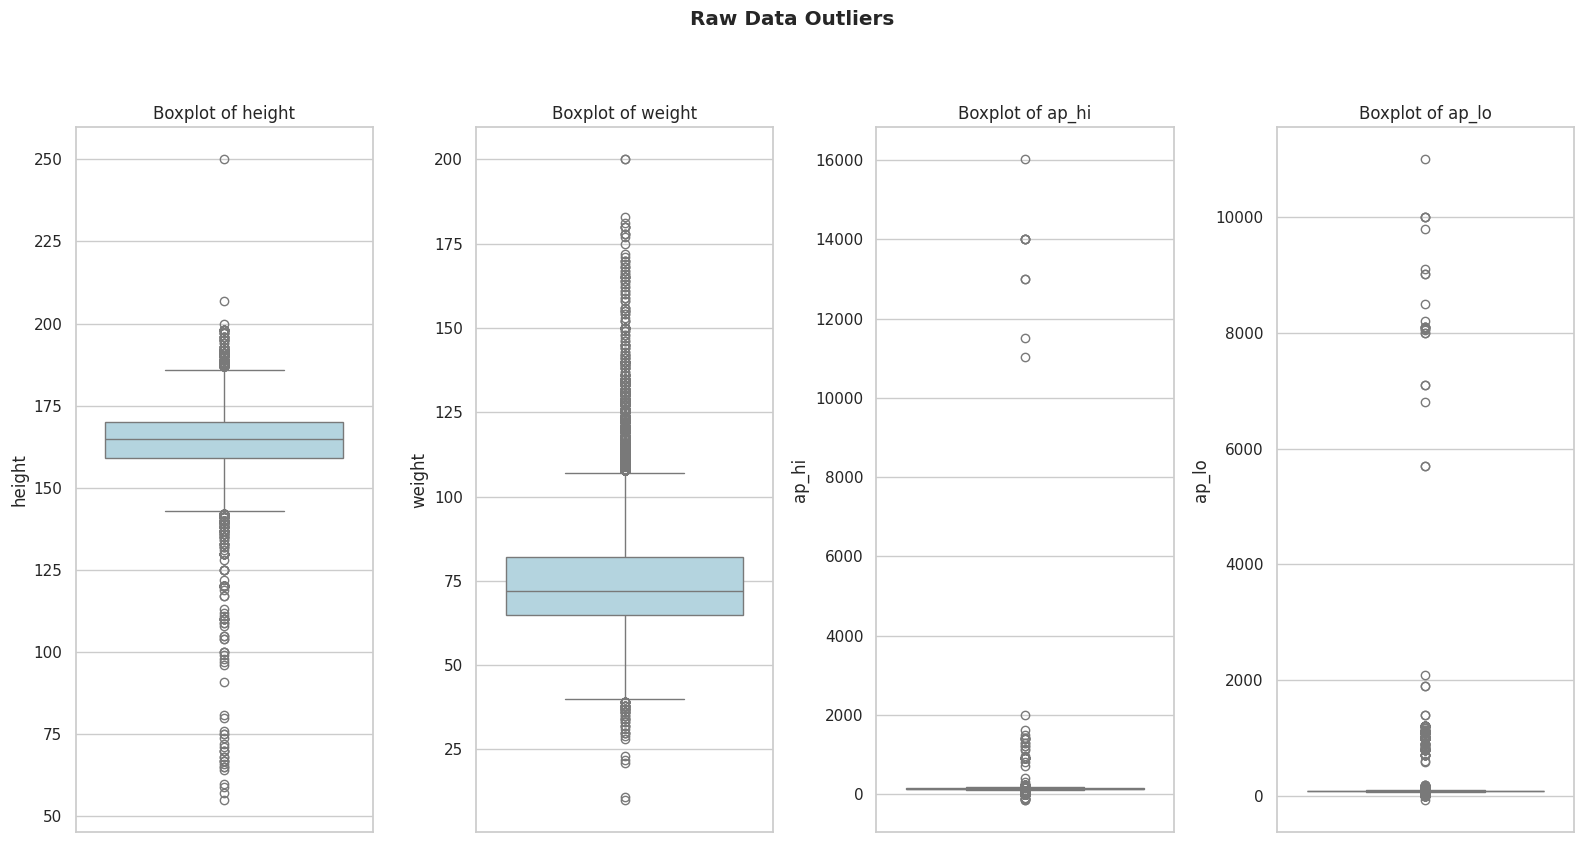
\includegraphics[width=0.94\textwidth,height=0.67\textheight,keepaspectratio]{raw_boxplots.png}
\caption{Raw-data boxplots used to diagnose extreme values before preprocessing.}
\label{fig:raw_boxplots}
\end{figure}

\begin{table}[htbp]
\centering
\small
\begin{tabularx}{\textwidth}{@{}lXrr@{}}
\toprule
\textbf{Step} & \textbf{Rule} & \textbf{Affected} & \textbf{Remaining}\\
\midrule
Duplicate removal & Remove duplicated clinical records & 24 dropped & 69,976\\
Negative BP correction & Absolute value under sign-error assumption & 8 corrected & 69,976\\
Inconsistent BP & Remove \code{ap\_lo} $\geq$ \code{ap\_hi} & 1,230 dropped & 68,746\\
Height range & Keep $[125,215]$ cm & 85 dropped & 68,661\\
Weight range & Keep $[40,200]$ kg & 48 dropped & 68,613\\
Systolic BP range & Keep $[70,250]$ mmHg & 45 dropped & 68,568\\
Diastolic BP range & Keep $[40,150]$ mmHg & 51 dropped & 68,517\\
\bottomrule
\end{tabularx}
\caption{Sequential preprocessing and data-quality treatment.}
\label{tab:preprocessing}
\end{table}

EDA was performed on the cleaned dataset. The final target remained balanced: 34,609 Class~0 observations (50.51\%) and 33,908 Class~1 observations (49.49\%), corresponding to a ratio of approximately 1.02:1. No imbalance-specific resampling was therefore used.

\begin{figure}[htbp]
\centering
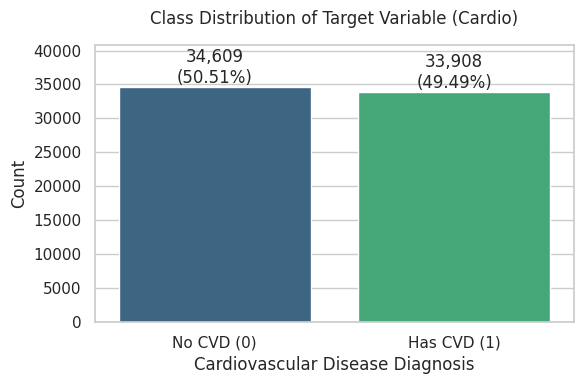
\includegraphics[width=0.94\textwidth,height=0.67\textheight,keepaspectratio]{class_distribution.png}
\caption{Class distribution after preprocessing.}
\label{fig:class_distribution}
\end{figure}

The principal continuous variables had the distributions shown in Table~\ref{tab:desc}. Age was concentrated in the older adult range represented by the dataset, weight was positively skewed, and blood-pressure values displayed clustering around commonly recorded values.

\begin{table}[H]
\centering
\small
\begin{tabular}{lrrrrrrr}
\toprule
\textbf{Feature} & \textbf{Mean} & \textbf{SD} & \textbf{Min} & \textbf{25\%} & \textbf{Median} & \textbf{75\%} & \textbf{Max}\\
\midrule
\code{age\_years} & 53.29 & 6.76 & 29.56 & 48.34 & 53.94 & 58.38 & 64.92\\
\code{height} & 164.44 & 7.85 & 125.00 & 159.00 & 165.00 & 170.00 & 207.00\\
\code{weight} & 74.14 & 14.27 & 40.00 & 65.00 & 72.00 & 82.00 & 200.00\\
\code{ap\_hi} & 126.68 & 16.68 & 70.00 & 120.00 & 120.00 & 140.00 & 240.00\\
\code{ap\_lo} & 81.31 & 9.42 & 40.00 & 80.00 & 80.00 & 90.00 & 150.00\\
\bottomrule
\end{tabular}
\caption{Descriptive statistics after preprocessing.}
\label{tab:desc}
\end{table}

\begin{figure}[htbp]
\centering
\begin{subfigure}{0.94\textwidth}
\centering
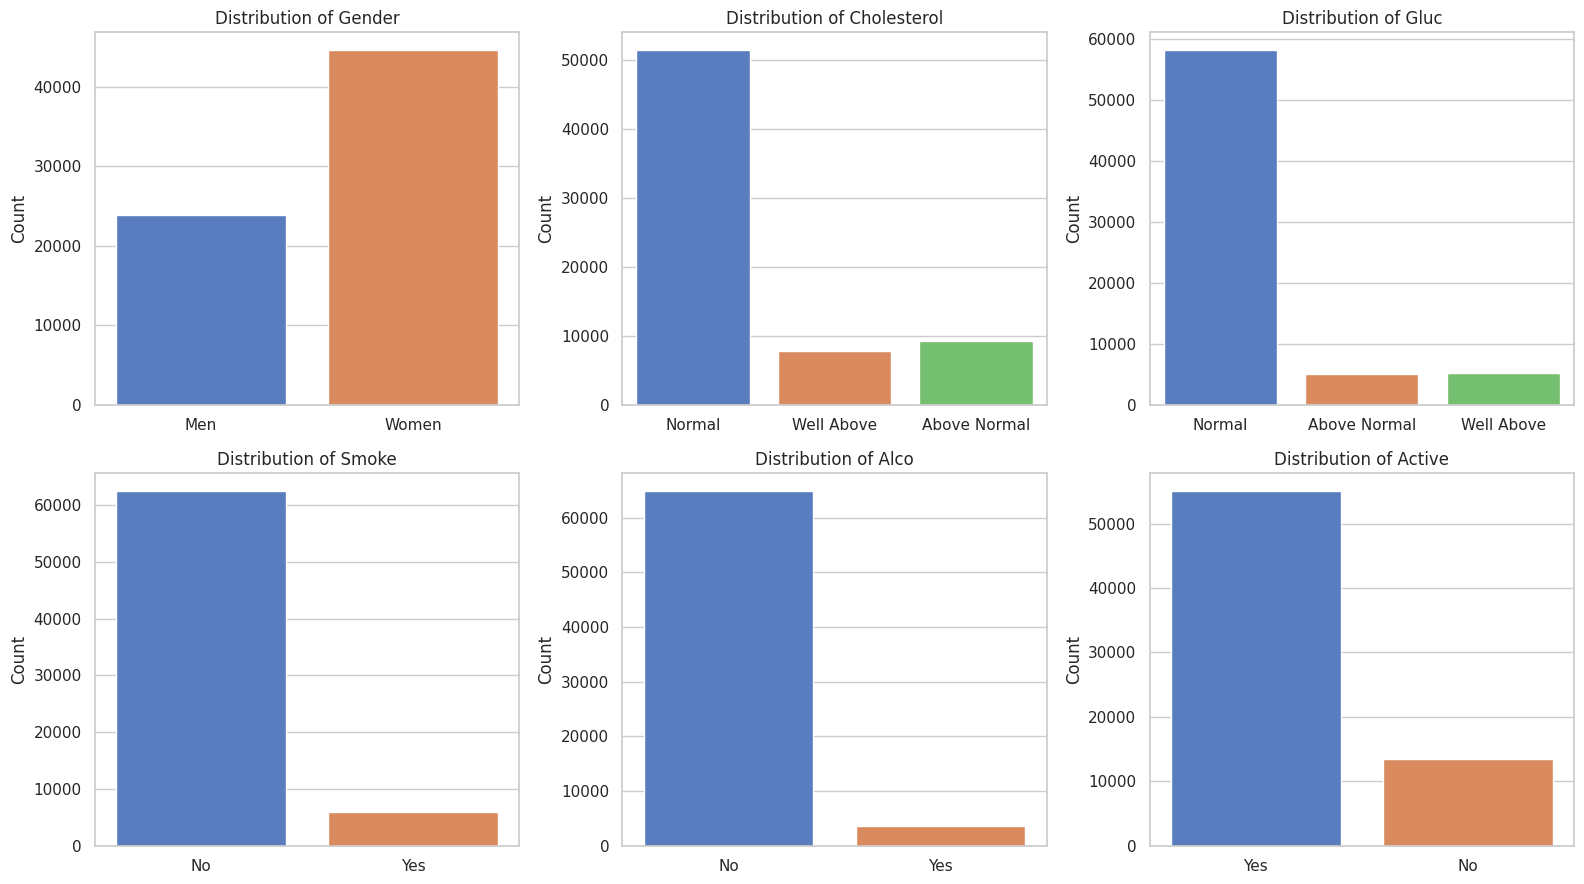
\includegraphics[width=\linewidth,height=0.36\textheight,keepaspectratio]{categorical_distributions.png}
\caption{Categorical and binary distributions.}
\end{subfigure}
\par\medskip
\begin{subfigure}{0.94\textwidth}
\centering
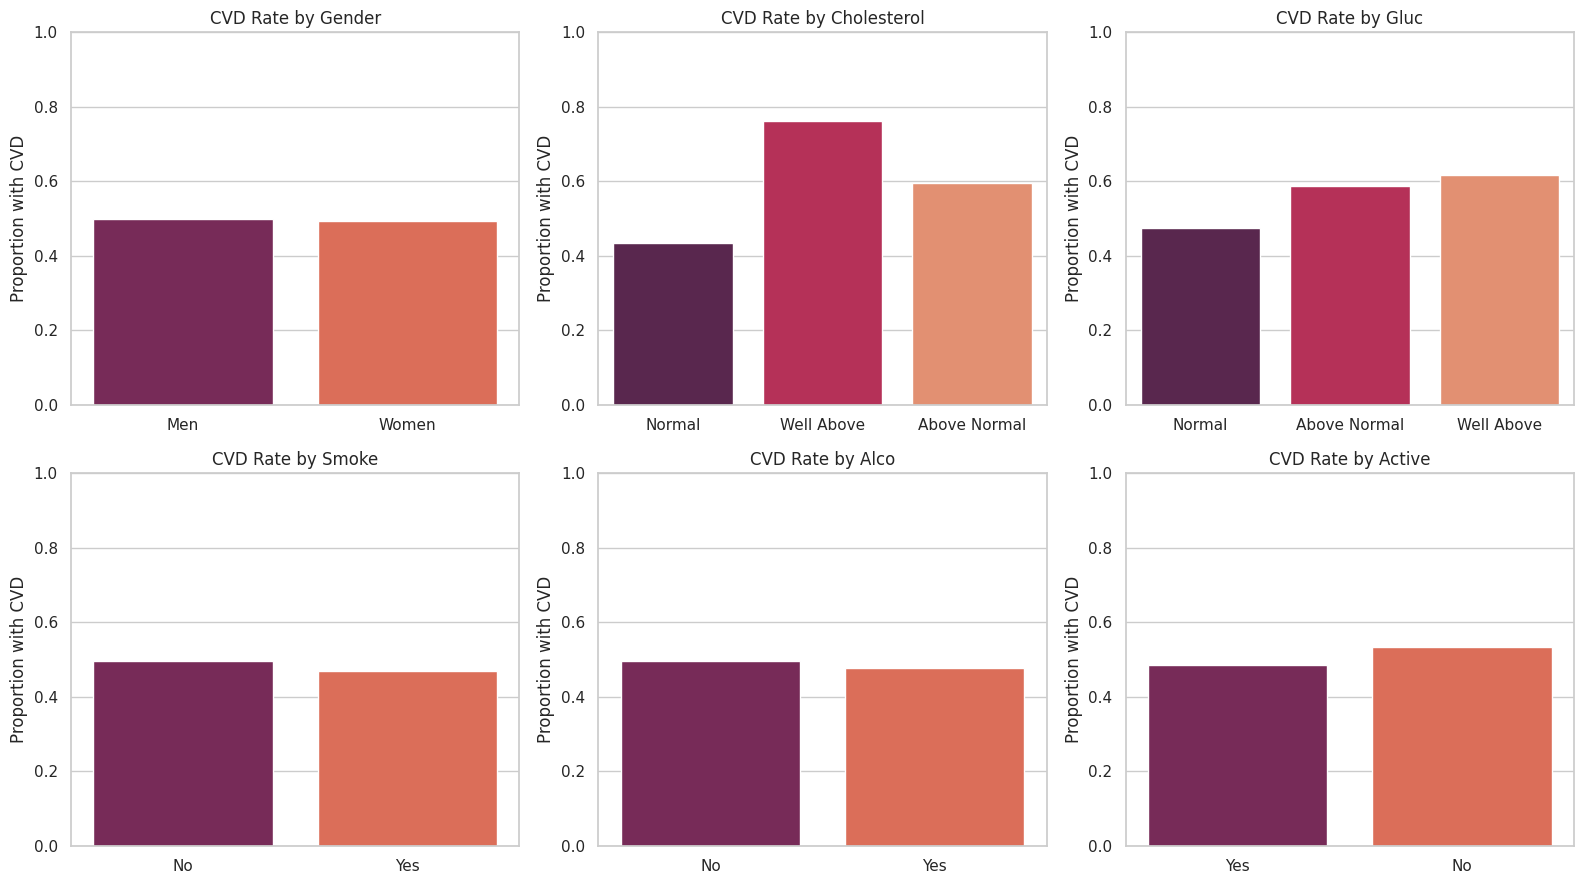
\includegraphics[width=\linewidth,height=0.36\textheight,keepaspectratio]{categorical_cvd_proportion.png}
\caption{Observed CVD proportion by group.}
\end{subfigure}
\caption{Categorical-variable distributions and observed CVD proportions.}
\label{fig:categorical}
\end{figure}

Women constituted 65.11\% of the cleaned data. Normal cholesterol and glucose categories dominated the dataset, while smoking and alcohol use were relatively infrequent. Elevated cholesterol and glucose showed stronger univariate separation by CVD status than gender, smoking, or alcohol intake.

\begin{figure}[htbp]
\centering
\begin{subfigure}{0.94\textwidth}
\centering
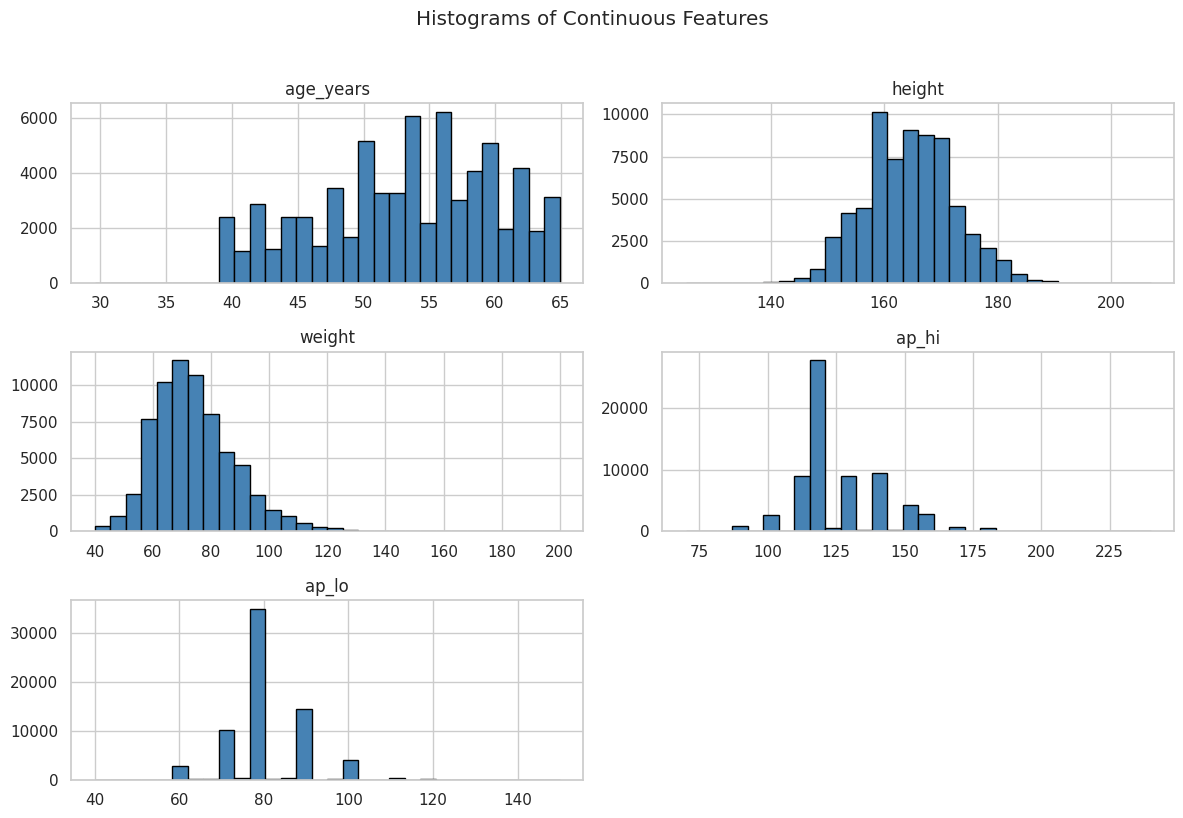
\includegraphics[width=\linewidth,height=0.36\textheight,keepaspectratio]{continuous_histograms.png}
\caption{Continuous-feature histograms.}
\end{subfigure}
\par\medskip
\begin{subfigure}{0.94\textwidth}
\centering
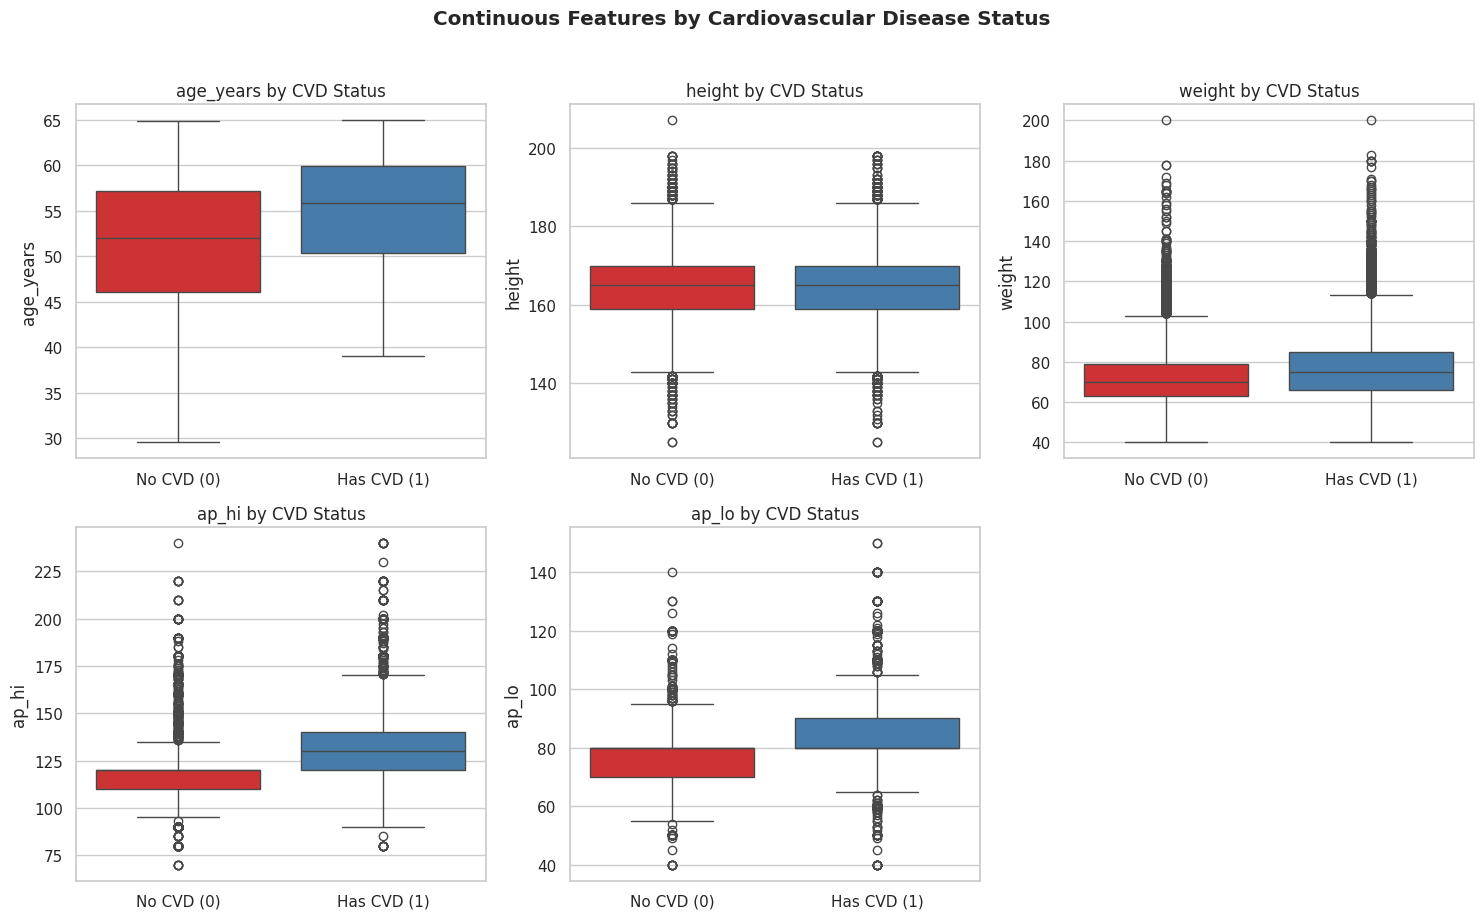
\includegraphics[width=\linewidth,height=0.36\textheight,keepaspectratio]{continuous_by_cvd.png}
\caption{Continuous features by CVD status.}
\end{subfigure}
\caption{Continuous-variable distributions after preprocessing.}
\label{fig:continuous_eda}
\end{figure}

Patients with CVD generally had higher age, weight, and blood-pressure distributions, although substantial overlap remained between classes. Pearson analysis identified a strong positive relationship between systolic and diastolic pressure ($r=0.73$). Among the original predictors, \code{ap\_hi} had the strongest linear association with the target ($r=0.43$), followed by \code{ap\_lo} ($r=0.34$), age ($r=0.24$), and cholesterol ($r=0.22$). These are pairwise linear associations rather than causal effects.

\begin{figure}[htbp]
\centering
\begin{subfigure}{\textwidth}
\centering
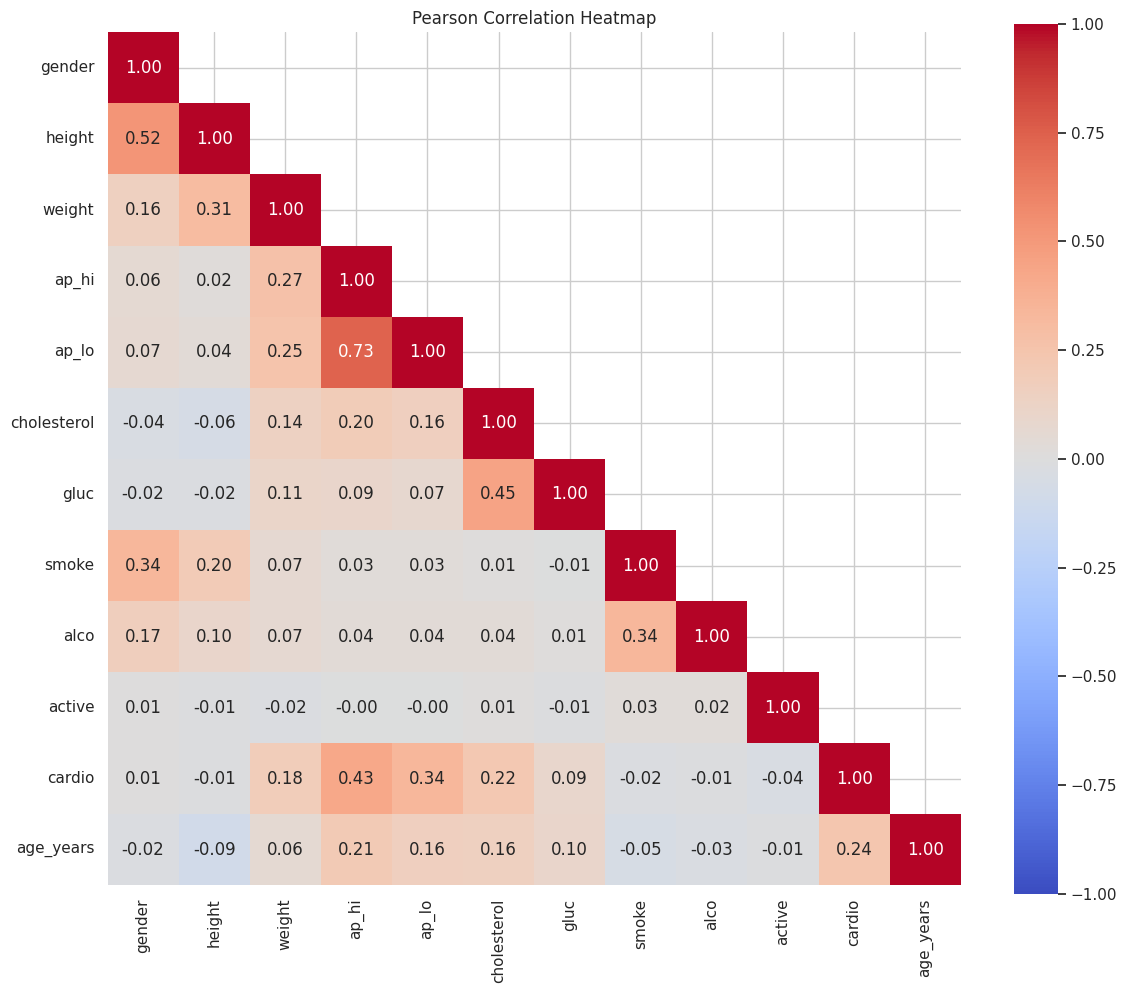
\includegraphics[width=\linewidth,height=0.36\textheight,keepaspectratio]{correlation_heatmap.png}
\caption{Pearson correlation heatmap.}
\end{subfigure}
\par\medskip
\begin{subfigure}{\textwidth}
\centering
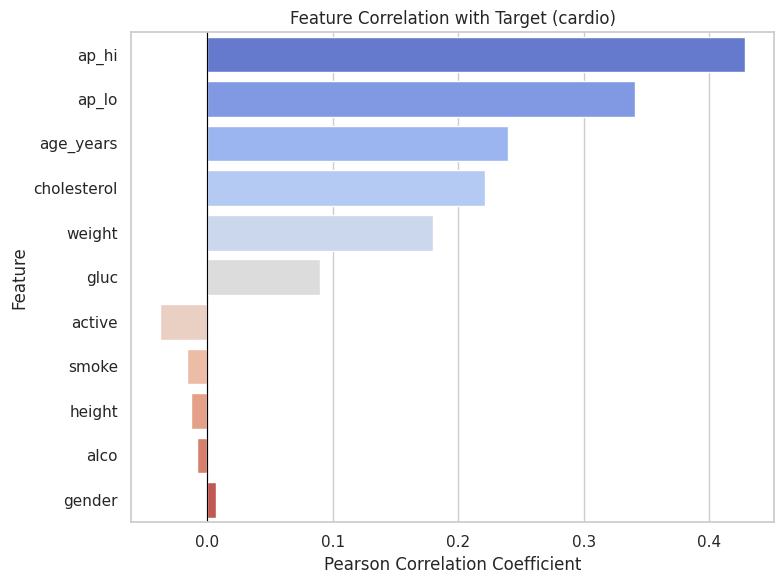
\includegraphics[width=\linewidth,height=0.36\textheight,keepaspectratio]{target_correlations.png}
\caption{Correlations with \code{cardio}.}
\end{subfigure}
\caption{Correlation analysis of the cleaned predictors.}
\label{fig:correlation}
\end{figure}

No exact duplicate rows remained after preprocessing. Thirty-four records formed 17 conflicting predictor profiles with opposite target labels. These profiles indicate that the observed variables do not completely determine CVD status and may reflect unmeasured clinical factors, temporal differences, diagnostic uncertainty, or label noise. IQR diagnostics also identified observations outside conventional statistical fences (e.g., 3,483 for diastolic pressure), but these were retained when they remained inside the adopted plausibility thresholds.

\subsection{Engineered-Feature Observations}

The engineered dataset contained 68,517 records and 23 columns (22 predictors plus the target). Figure~\ref{fig:engineered_features} illustrates representative engineered features. BMI, pulse pressure, and MAP were generally shifted upward among CVD cases, whereas the lifestyle-risk score showed weaker standalone class separation.

\begin{figure}[htbp]
\centering
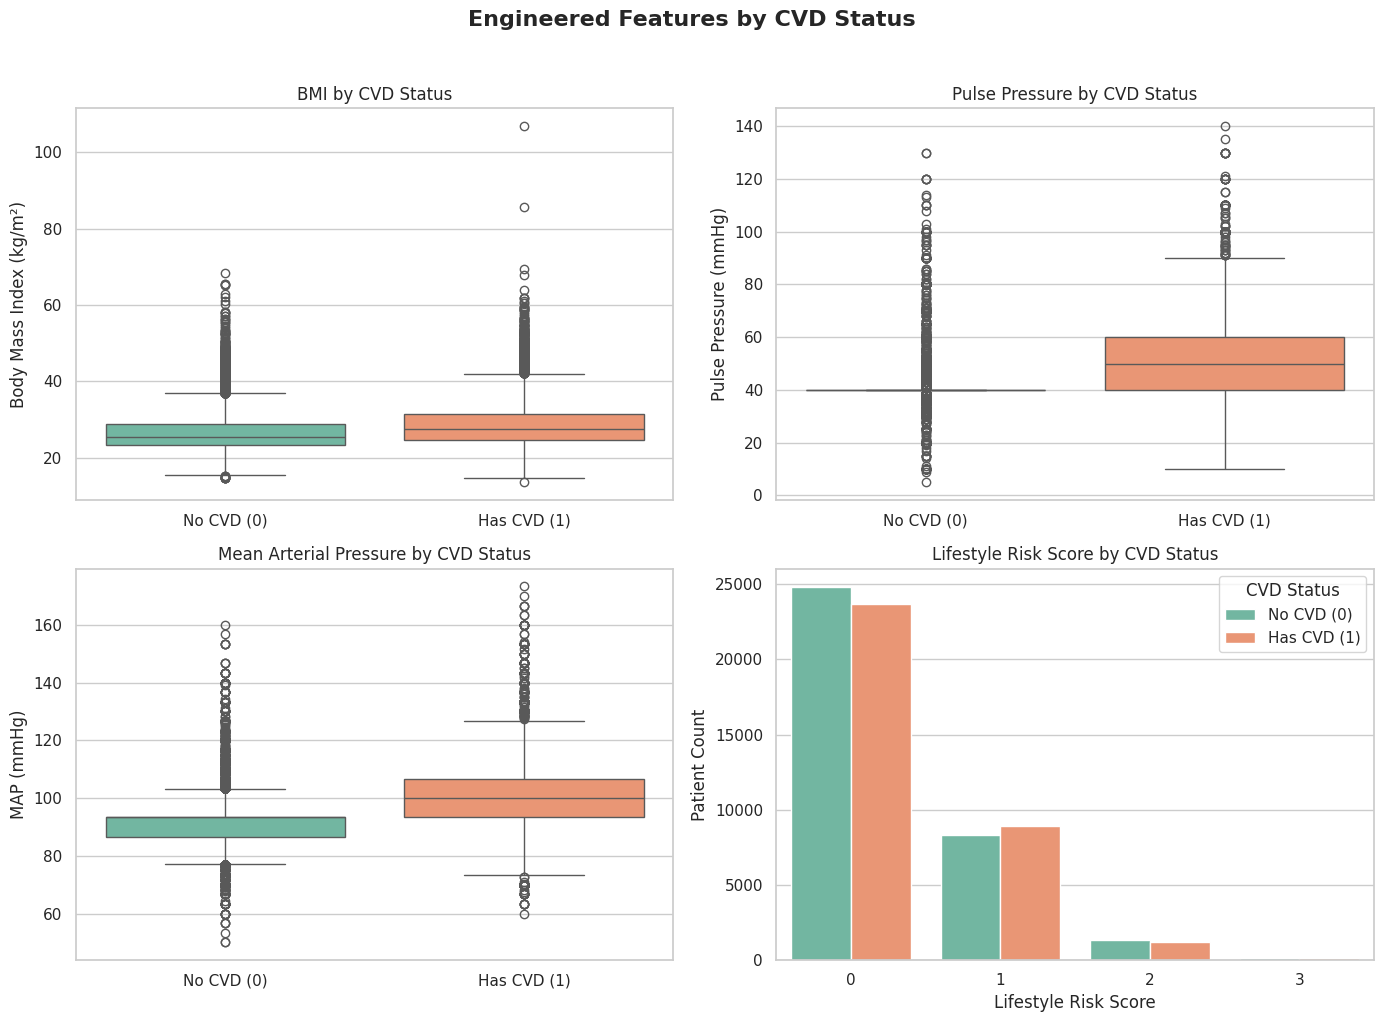
\includegraphics[width=0.94\textwidth,height=0.67\textheight,keepaspectratio]{engineered_features.png}
\caption{Representative engineered features by CVD status.}
\label{fig:engineered_features}
\end{figure}

\subsection{Feature Selection Results}

\begin{table}[htbp]
\centering
\small
\begin{tabular}{lcc}
\toprule
\textbf{Feature subset} & \textbf{\# predictors} & \textbf{Mean CV accuracy}\\
\midrule
Original only & 11 & 72.72\% ($\pm$0.34\%)\\
Engineered only & 11 & 72.59\% ($\pm$0.43\%)\\
All original + engineered & 22 & 72.82\% ($\pm$0.28\%)\\
Top-5 ANOVA & 5 & 71.28\% ($\pm$0.51\%)\\
Top-5 Mutual Information & 5 & 71.28\% ($\pm$0.51\%)\\
Top-5 RFE & 5 & 72.82\% ($\pm$0.53\%)\\
\bottomrule
\end{tabular}
\caption{Feature-subset comparison on the training partition.}
\label{tab:feature_subsets}
\end{table}

The final predictors were \code{ap\_hi},
\code{age\_cholesterol\_interaction}, \code{age\_years},
\code{bmi}, and \code{map}. 

The engineered-only representation achieved 72.5905\% mean
cross-validation accuracy, compared with 72.7200\% for the original
features. Engineering alone therefore did not improve the reference
classifier. Combining original and engineered variables increased
mean accuracy to 72.8221\%, a modest gain of approximately 0.1022
percentage points.

The RFE pipeline achieved 72.8203\% with five predictors. This was
approximately 0.0018 percentage points below the complete representation,
so both results rounded to 72.82\%. The principal descriptive benefit
was substantial dimensionality reduction with almost unchanged mean
validation accuracy, rather than an established accuracy improvement.

The age--cholesterol interaction was retained and became the
second-ranked feature in the subsequent SHAP analyses. This supports
its usefulness within the fitted representation, but no individual
feature-ablation experiment was performed to isolate its incremental
benefit. ANOVA and Mutual Information selected several related
blood-pressure features, and their five-feature subsets achieved
approximately 71.28\% accuracy.

\subsection{Individual Model Tuning}

Table~\ref{tab:tuning} reports the four required configurations for each individual classifier. The shallowest Decision Tree performed best, with validation accuracy decreasing as depth increased. For the SVM, the RBF kernel achieved the highest mean validation accuracy.

\begin{table}[htbp]
\centering
\small
\begin{tabular}{lc|lc}
\toprule
\multicolumn{2}{c|}{\textbf{Decision Tree}} & \multicolumn{2}{c}{\textbf{SVM}}\\
\textbf{Depth} & \textbf{CV accuracy} & \textbf{Kernel} & \textbf{CV accuracy}\\
\midrule
5 & 72.97\% ($\pm$0.44\%) & Linear & 72.51\% ($\pm$0.37\%)\\
10 & 72.26\% ($\pm$0.38\%) & Polynomial & 68.68\% ($\pm$0.39\%)\\
15 & 70.36\% ($\pm$0.46\%) & RBF & 73.18\% ($\pm$0.35\%)\\
20 & 68.38\% ($\pm$0.53\%) & Sigmoid & 64.77\% ($\pm$0.38\%)\\
\bottomrule
\end{tabular}
\caption{Five-fold validation performance of the required hyperparameter configurations.}
\label{tab:tuning}
\end{table}

\begin{figure}[htbp]
\centering
\begin{subfigure}{0.94\textwidth}
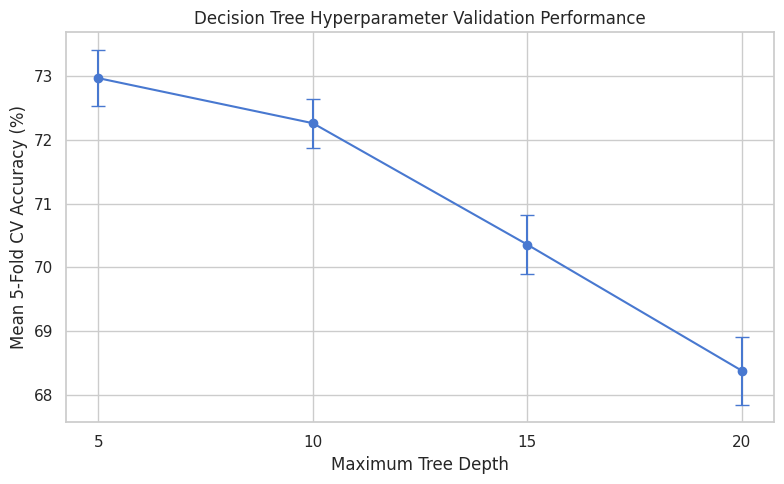
\includegraphics[width=\linewidth,height=0.36\textheight,keepaspectratio]{dt_validation_performance.png}
\caption{Decision Tree depth validation.}
\end{subfigure}
\par\medskip
\begin{subfigure}{0.94\textwidth}
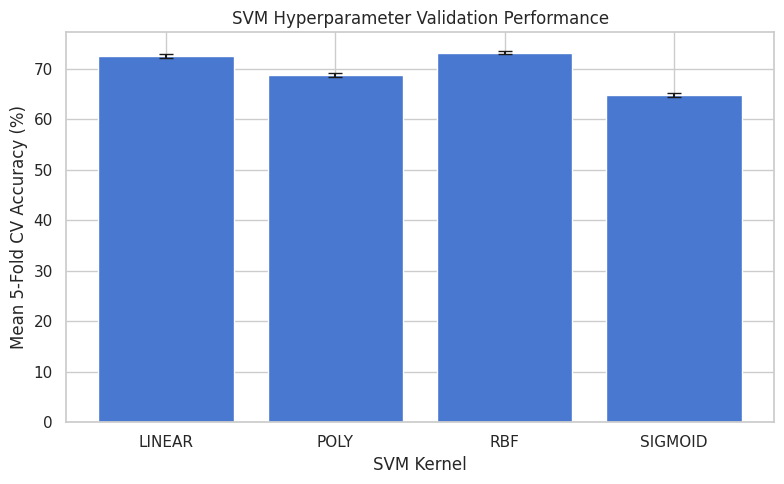
\includegraphics[width=\linewidth,height=0.36\textheight,keepaspectratio]{svm_validation_performance.png}
\caption{SVM kernel validation.}
\end{subfigure}
\caption{Validation performance for the four configurations of each individual model.}
\label{fig:validation_performance}
\end{figure}

\subsection{Ensemble Selection Results}

Soft Voting achieved fold accuracies of 73.32\%, 72.82\%, 72.85\%, 73.99\%, and 73.39\%, giving a mean of 73.27\% ($\pm$0.43\%). The Stacking candidate obtained 73.05\%, 72.75\%, 72.61\%, 73.99\%, and 72.97\%, for a mean of 73.07\% ($\pm$0.48\%). Soft Voting was higher in four folds and equal in one.

\begin{figure}[htbp]
\centering
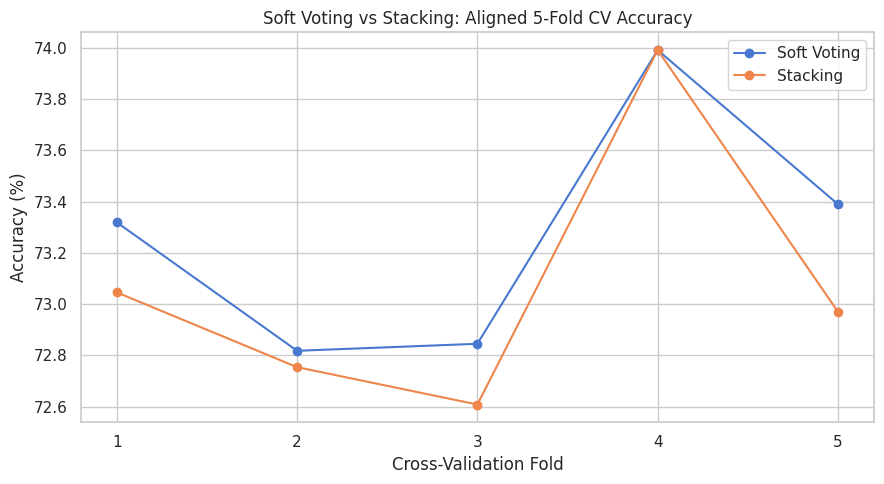
\includegraphics[width=0.94\textwidth,height=0.67\textheight,keepaspectratio]{ensemble_selection_cv.png}
\caption{Aligned five-fold accuracy used to select between Soft Voting and Stacking.}
\label{fig:ensemble_selection}
\end{figure}

Soft Voting was therefore selected as the final ensemble using training cross-validation only. The Stacking model was not evaluated on the held-out test set after it lost the pre-specified ensemble-selection comparison. This prevented the test partition from becoming a second model-selection dataset.

\subsection{Held-out Test Performance}

Table~\ref{tab:test_metrics} summarises final test performance. The SVM achieved the highest accuracy, precision, specificity, MCC, and Kappa. The Decision Tree had the highest recall among the two individual classifiers. Soft Voting achieved the highest F1-score, ROC-AUC, and Average Precision, while its accuracy was only 0.02 percentage points below the SVM.

\begin{table}[H]
\centering
\small
\begin{tabularx}{\textwidth}{@{}lXXX@{}}
\toprule
\textbf{Metric} & \textbf{Decision Tree} & \textbf{SVM (RBF)} & \textbf{Soft Voting}\\
\midrule
Accuracy & 73.18\% & \textbf{73.47\%} & 73.45\%\\
Precision & 74.85\% & \textbf{76.02\%} & 75.65\%\\
Recall & \textbf{68.98\%} & 67.77\% & 68.34\%\\
Specificity & 77.29\% & \textbf{79.05\%} & 78.45\%\\
F1-score & 71.79\% & 71.66\% & \textbf{71.81\%}\\
ROC-AUC & 0.7914 & 0.7827 & \textbf{0.7935}\\
Average Precision & 0.7626 & 0.7661 & \textbf{0.7756}\\
MCC & 0.4644 & \textbf{0.4714} & 0.4705\\
Cohen's Kappa & 0.4630 & \textbf{0.4687} & 0.4683\\
\bottomrule
\end{tabularx}
\caption{Held-out test performance of the final models.}
\label{tab:test_metrics}
\end{table}

The corresponding confusion matrices were:
\begin{itemize}
    \item Decision Tree: TN = 5,350, FP = 1,572, FN = 2,104, TP = 4,678;
    \item SVM: TN = 5,472, FP = 1,450, FN = 2,186, TP = 4,596;
    \item Soft Voting: TN = 5,430, FP = 1,492, FN = 2,147, TP = 4,635.
\end{itemize}

\begin{figure}[htbp]
\centering
\begin{subfigure}{0.94\textwidth}
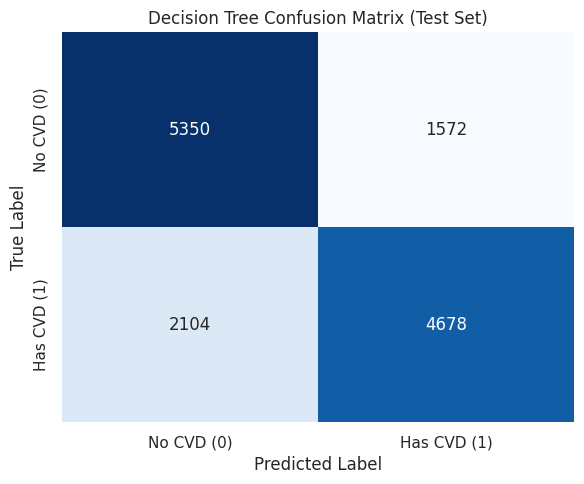
\includegraphics[width=\linewidth,height=0.22\textheight,keepaspectratio]{dt_confusion_matrix.png}
\caption{Decision Tree.}
\end{subfigure}
\par\medskip
\begin{subfigure}{0.94\textwidth}
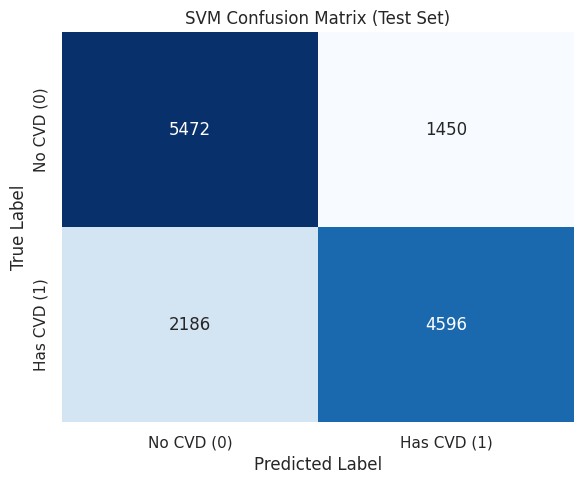
\includegraphics[width=\linewidth,height=0.22\textheight,keepaspectratio]{svm_confusion_matrix.png}
\caption{SVM.}
\end{subfigure}
\par\medskip
\begin{subfigure}{0.94\textwidth}
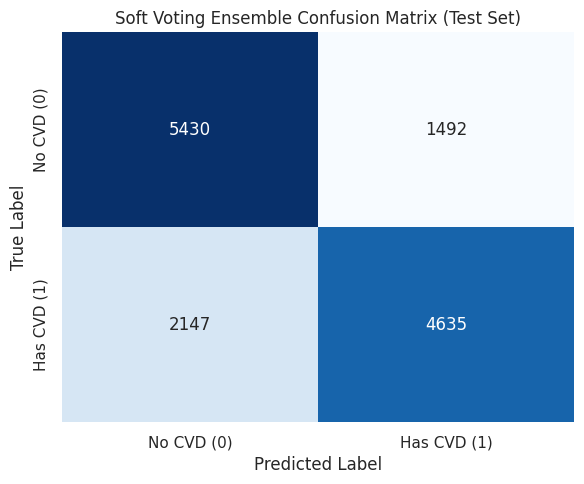
\includegraphics[width=\linewidth,height=0.22\textheight,keepaspectratio]{soft_confusion_matrix.png}
\caption{Soft Voting.}
\end{subfigure}
\caption{Confusion matrices on the held-out test set.}
\label{fig:confusions}
\end{figure}

\begin{figure}[htbp]
\centering
\begin{subfigure}{0.94\textwidth}
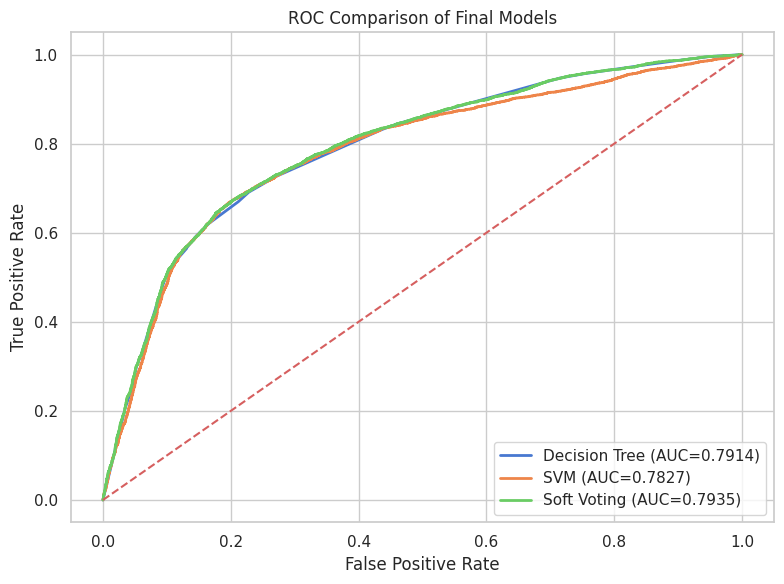
\includegraphics[width=\linewidth,height=0.36\textheight,keepaspectratio]{combined_roc_curves.png}
\caption{ROC curves.}
\end{subfigure}
\par\medskip
\begin{subfigure}{0.94\textwidth}
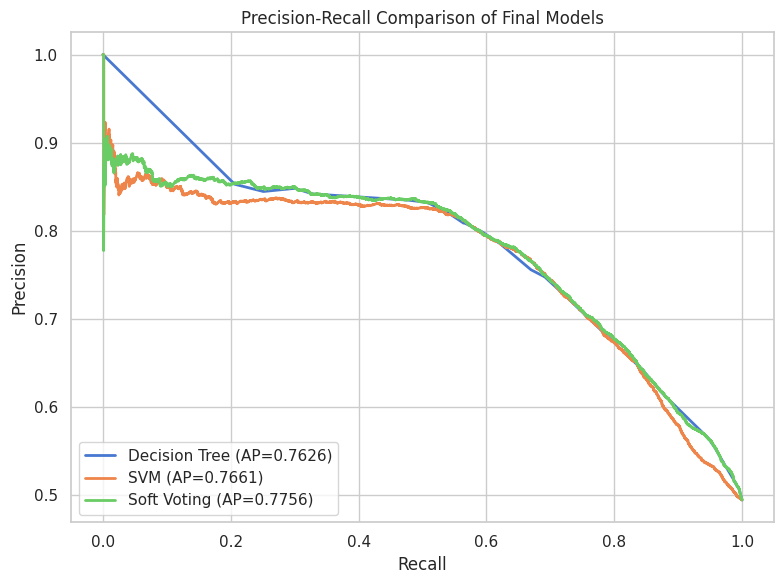
\includegraphics[width=\linewidth,height=0.36\textheight,keepaspectratio]{combined_pr_curves.png}
\caption{Precision--Recall curves.}
\end{subfigure}
\caption{Probability-ranking comparison of the final models.}
\label{fig:roc_pr}
\end{figure}

\subsection{Decision Tree Feature Importance}

The fitted depth-5 Decision Tree's Gini importance was strongly concentrated on systolic blood pressure (78.33\%), followed by the age--cholesterol interaction (17.14\%), age (3.12\%), BMI (0.98\%), and MAP (0.44\%).

\begin{figure}[htbp]
\centering
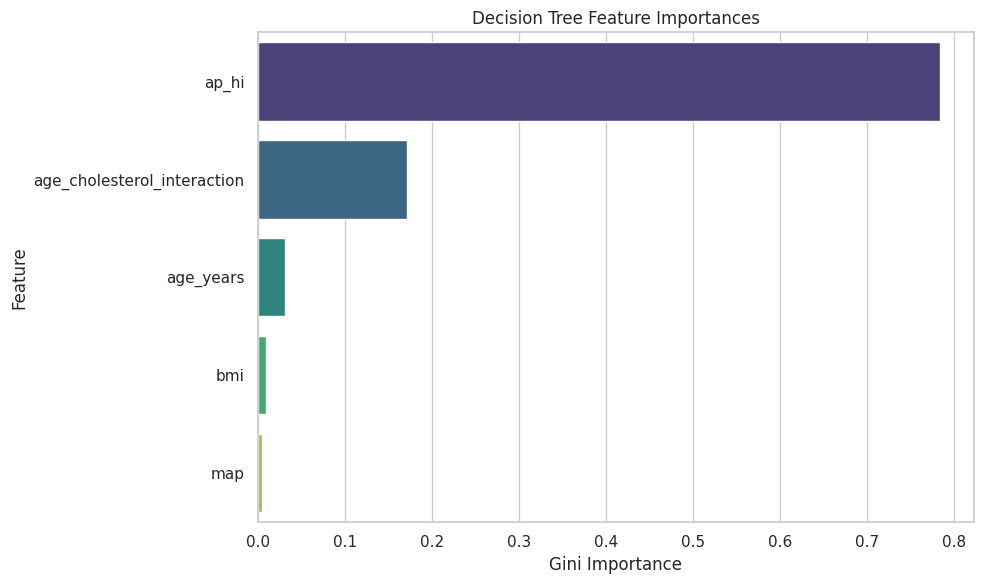
\includegraphics[width=0.94\textwidth,height=0.67\textheight,keepaspectratio]{dt_feature_importance.png}
\caption{Gini feature importance of the final Decision Tree.}
\label{fig:dt_importance}
\end{figure}

\subsection{Global SHAP Results}

Permutation SHAP produced the same global feature ranking for all three models:
\begin{enumerate}
    \item \code{ap\_hi};
    \item \code{age\_cholesterol\_interaction};
    \item \code{age\_years};
    \item \code{map}; and
    \item \code{bmi}.
\end{enumerate}

Table~\ref{tab:shap_values} reports the mean absolute SHAP magnitudes. The Decision Tree concentrated most heavily on systolic pressure, whereas the SVM distributed more attribution across age, MAP, and BMI. Soft Voting displayed an intermediate attribution profile, consistent with averaging the two model probabilities.

\begin{table}[htbp]
\centering
\small
\begin{tabularx}{\textwidth}{@{}Xrrr@{}}
\toprule
\textbf{Feature} & \textbf{Decision Tree} & \textbf{SVM} & \textbf{Soft Voting}\\
\midrule
\code{ap\_hi} & 0.174335 & 0.139499 & 0.156916\\
\code{age\_cholesterol\_interaction} & 0.073297 & 0.051680 & 0.054200\\
\code{age\_years} & 0.019206 & 0.046381 & 0.030493\\
\code{map} & 0.017447 & 0.034728 & 0.025920\\
\code{bmi} & 0.009955 & 0.018765 & 0.013807\\
\bottomrule
\end{tabularx}
\caption{Mean absolute SHAP values for the final models.}
\label{tab:shap_values}
\end{table}

\begin{figure}[H]
\centering
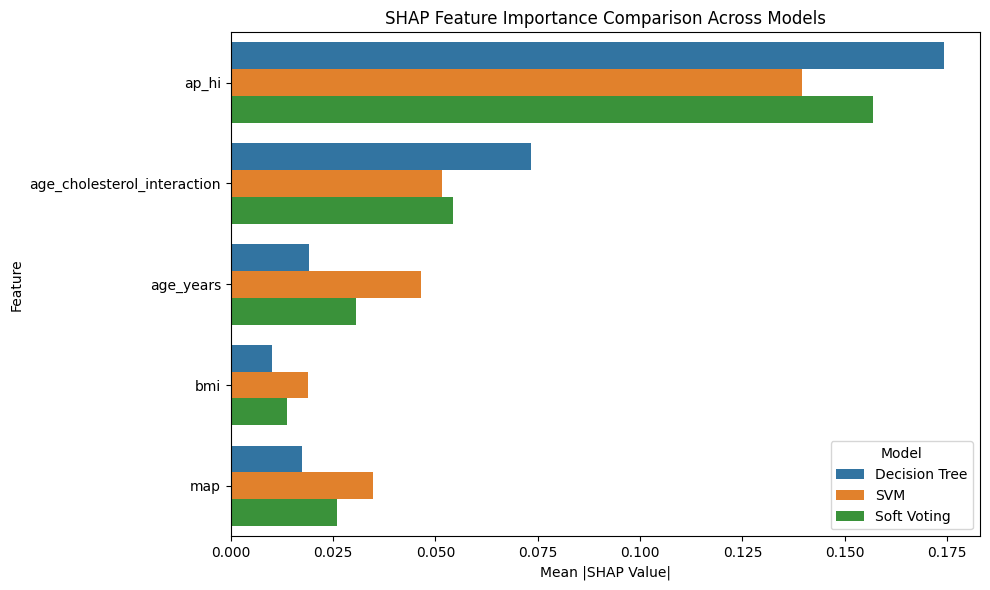
\includegraphics[width=0.94\textwidth,height=0.67\textheight,keepaspectratio]{shap_model_comparison.png}
\caption{Cross-model comparison of mean absolute SHAP values.}
\label{fig:shap_comparison}
\end{figure}

\begin{figure}[H]
\centering
\begin{subfigure}{0.9\textwidth}
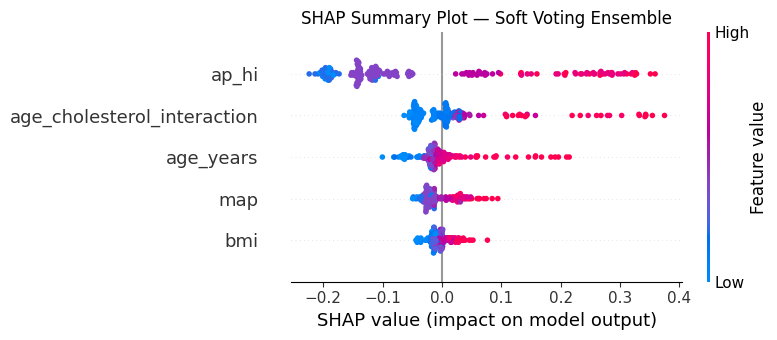
\includegraphics[width=\linewidth,height=0.24\textheight,keepaspectratio]{soft_shap_summary.png}
\caption{Soft Voting SHAP summary.}
\end{subfigure}
\par\medskip
\begin{subfigure}{0.9\textwidth}
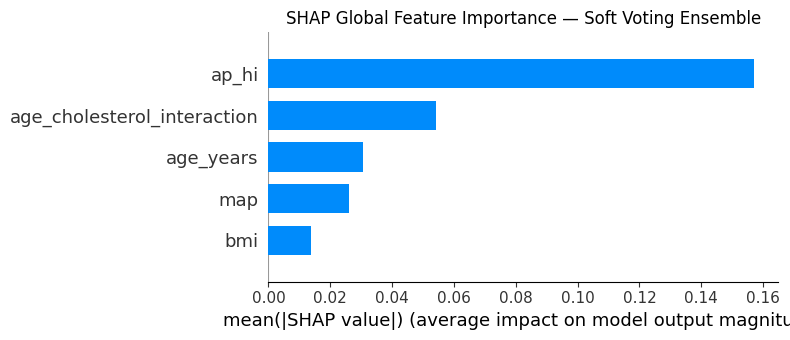
\includegraphics[width=\linewidth,height=0.24\textheight,keepaspectratio]{soft_shap_bar.png}
\caption{Soft Voting global bar plot.}
\end{subfigure}
\caption{Global SHAP explanations for the selected Soft Voting ensemble.}
\label{fig:soft_shap}
\end{figure}

The Soft Voting summary plot shows that higher \code{ap\_hi}, higher age--cholesterol interaction, greater age, and higher MAP generally push the predicted CVD probability upward, while lower values tend to reduce it. BMI has the smallest mean absolute contribution among the selected predictors.

\subsection{SHAP Dependence and Local Explanations}

The dependence plot for \code{ap\_hi} shows a nonlinear, step-like
relationship between systolic pressure and its attributed contribution
to the Soft Voting prediction. Values around and below 120~mmHg
generally contribute negatively, whereas higher values generally
contribute positively within the explanation sample. Colour displays
the age--cholesterol interaction feature selected by the plotting
routine. This visual association suggests variation across patient
profiles.

\begin{figure}[htbp]
\centering
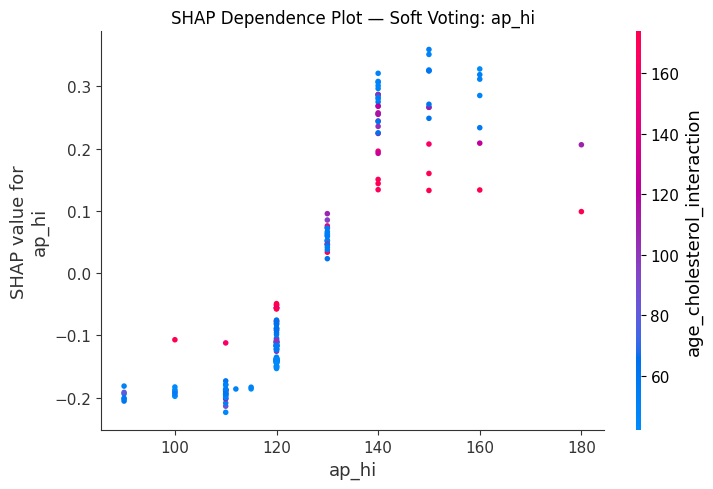
\includegraphics[width=0.8\textwidth,height=0.6\textheight,keepaspectratio]{soft_shap_dependence.png}
\caption{SHAP dependence plot for systolic blood pressure in the Soft Voting ensemble.}
\label{fig:shap_dependence}
\end{figure}

Two correctly classified cases were selected for local interpretation. The non-CVD case had $P(\mathrm{CVD}=1)=0.1934$. Its systolic pressure of 120~mmHg reduced the probability by approximately 0.15 from the background expectation, while younger age and the low age--cholesterol interaction also reduced the prediction. The CVD case had $P(\mathrm{CVD}=1)=0.7022$. Despite a low systolic pressure of 100~mmHg contributing approximately $-0.11$, its very high age--cholesterol interaction contributed approximately $+0.38$, dominating the final prediction. This example demonstrates why local explanations are useful: a positive classification need not be driven by the globally strongest variable in every patient.

\begin{figure}[H]
\centering
\begin{subfigure}{0.8\textwidth}
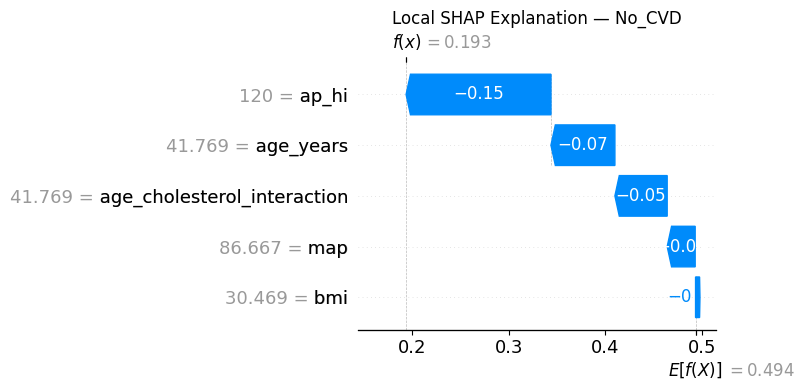
\includegraphics[width=\linewidth,height=0.24\textheight,keepaspectratio]{local_no_cvd.png}
\caption{Correctly classified non-CVD patient.}
\end{subfigure}
\par\medskip
\begin{subfigure}{0.8\textwidth}
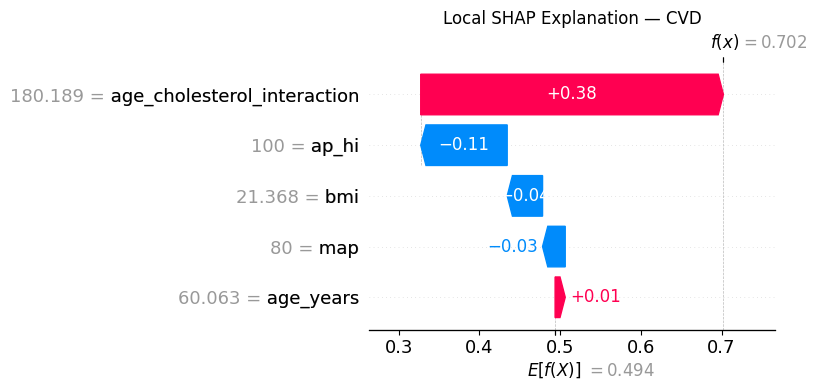
\includegraphics[width=\linewidth,height=0.24\textheight,keepaspectratio]{local_cvd.png}
\caption{Correctly classified CVD patient.}
\end{subfigure}
\caption{Local SHAP waterfall explanations for two held-out patients.}
\label{fig:local_shap}
\end{figure}

\subsection{Statistical Comparison}

The aligned fold scores used for statistical testing are reported in Table~\ref{tab:paired_folds}. Soft Voting improved over the Decision Tree in every fold. Relative to the SVM, the ensemble was better in four folds and slightly worse in one.

\begin{table}[H]
\centering
\small
\begin{tabular}{crrr}
\toprule
\textbf{Fold} & \textbf{Decision Tree} & \textbf{SVM} & \textbf{Soft Voting}\\
\midrule
1 & 0.730183 & 0.732737 & 0.733193\\
2 & 0.726352 & 0.728724 & 0.728177\\
3 & 0.725440 & 0.728177 & 0.728450\\
4 & 0.737822 & 0.737822 & 0.739920\\
5 & 0.728517 & 0.731436 & 0.733899\\
\midrule
Mean & 0.729663 & 0.731779 & 0.732728\\
\bottomrule
\end{tabular}
\caption{Aligned five-fold accuracy scores used for paired statistical testing.}
\label{tab:paired_folds}
\end{table}

For Soft Voting versus the Decision Tree, the mean improvement was 0.3065 percentage points. Shapiro--Wilk testing of the five paired differences produced $W=0.8512$, $p=0.1982$, so normality was not rejected under the required decision rule. The one-sided paired $t$-test produced $t=4.8924$, $p=0.0040$. The null hypothesis was rejected: there is statistically significant evidence, under this five-fold analysis, that Soft Voting achieves greater cross-validation accuracy than the Decision Tree.

For Soft Voting versus the SVM, the mean improvement was only 0.0949 percentage points. Shapiro--Wilk produced $W=0.9097$, $p=0.4657$, and the one-sided paired $t$-test produced $t=1.6577$, $p=0.0864$. The null hypothesis was not rejected at $\alpha=0.05$. Therefore, there is insufficient evidence that Soft Voting improves upon the SVM.

\begin{table}[htbp]
\centering
\small
\begin{tabularx}{\textwidth}{@{}lrrrrX@{}}
\toprule
\textbf{Comparison} & \textbf{Mean gain (pp)} & \textbf{Shapiro $p$} & \textbf{$t$} & \textbf{$p$} & \textbf{Conclusion}\\
\midrule
Soft Voting vs DT & 0.3065 & 0.1982 & 4.8924 & 0.0040 & Significant improvement; reject $H_0$.\\
Soft Voting vs SVM & 0.0949 & 0.4657 & 1.6577 & 0.0864 & Not significant; fail to reject $H_0$.\\
\bottomrule
\end{tabularx}
\caption{Paired statistical comparison of the selected ensemble against the individual classifiers.}
\label{tab:stats}
\end{table}

\section{Discussion}

\subsection{Model Performance and Error Trade-offs}

The best model depends on the evaluation criterion. The SVM had the highest held-out accuracy (73.47\%), precision, and specificity, whereas Soft Voting had the highest F1-score (71.81\%), ROC-AUC (0.7935), and Average Precision (0.7756). The 0.02-percentage-point accuracy difference is small and does not establish a practically decisive separation.

The SVM produced the fewest false positives and therefore the highest specificity, but it also produced the most false negatives and lowest recall. The Decision Tree made the opposite trade-off, recovering more positive cases at the cost of more false positives. Soft Voting lay between the two and achieved the strongest F1-score. This is consistent with probability averaging moderating the decision behaviour of the two components.



Although the three models had nearly identical accuracy, the ROC and precision--recall results show that Soft Voting produced the strongest ranking performance. This distinction is important because a single threshold-based accuracy value does not fully characterise the quality of model probabilities.

The shallower tree's stronger validation performance is consistent with deeper trees fitting patterns that generalise less well. This is an interpretation of the validation trend; a training-versus-validation learning-curve analysis would be needed to examine that explanation directly. The RBF kernel gave the strongest tested SVM configuration, suggesting that a nonlinear boundary was useful among the four configurations evaluated.

\subsection{Effects of Feature Engineering and Selection}

The engineered-only representation did not improve on the original predictors. Combining both sets produced a small descriptive gain, while RFE retained near-identical mean validation accuracy with five rather than 22 predictors, reducing dimensionality by 77.3\%. The practical benefit was a compact representation rather than a demonstrated large accuracy increase.

BMI, MAP, and the age--cholesterol interaction were retained alongside age and systolic blood pressure. The interaction's high SHAP ranking indicates that the fitted models used it; without an individual ablation experiment, this does not quantify how much accuracy that feature added. Likewise, the near-match between reduced and complete representations is not a formal equivalence test.

\subsection{Influential Features and Agreement with Domain Knowledge}

The agreement across different model families strengthens confidence that the ranking is not merely an artefact of one classifier. It is also broadly consistent with domain knowledge: blood pressure is a major cardiovascular factor \cite{whelton2018}, age is clinically relevant, cholesterol contributes to cardiovascular risk, and BMI represents adiposity-related risk \cite{whoObesity2025}. However, SHAP attribution remains a model explanation rather than evidence of causality.



The local examples show why a global ranking cannot describe every patient. One positive prediction was dominated by the age--cholesterol interaction despite a negative systolic-pressure contribution. This makes the fitted decision more transparent, while the ordinal coding and correlated derived variables require care: attribution may be distributed across related representations, and agreement among models trained on the same predictors is not independent clinical validation.

\subsection{Did the Ensemble Significantly Improve Performance?}

Under the prescribed five-fold procedure, Soft Voting improved over the Decision Tree by 0.3065 percentage points on average ($p=0.0040$), but its 0.0949-percentage-point gain over the SVM was not significant ($p=0.0864$). Failure to reject the SVM comparison does not establish equivalence; it means this analysis did not demonstrate an improvement at $\alpha=0.05$.

Soft Voting was selected over Stacking using the training-CV criterion. The extra meta-learning stage did not improve that measured criterion in this experiment; no general superiority claim follows. The SVM remains a strong individual alternative, while the ensemble offers a modest improvement over the tree and stronger observed probability-ranking metrics.

\subsection{Limitations}

Several limitations constrain the interpretation of the results:
\begin{itemize}
    \item The dataset is cross-sectional and the target denotes observed disease status, so the models do not estimate prospective cardiovascular event risk.
    \item The dataset does not include many clinically important factors such as medication use, family history, waist circumference, detailed lipid measures, comorbidities, socioeconomic factors, or longitudinal history.
    \item Seventeen identical observed predictor profiles have conflicting labels, indicating imperfect separability from the available variables.
    \item The negative blood-pressure sign correction assumes data-entry sign errors because the original source does not document their cause.
    \item Project-defined plausibility thresholds and composite risk features are heuristics rather than validated clinical instruments.
    \item RFE used a Decision Tree reference estimator, which may bias the selected feature subset toward tree-compatible relationships.
    \item Equal-weight Soft Voting combines probability estimates from differently structured classifiers whose calibration characteristics may differ.
    \item SHAP was computed on a reproducible 200-record held-out sample for computational tractability rather than on all 13,704 test observations.
    \item Later model CV reused the feature subset selected on the complete training partition. These scores are conditional on that representation and are not nested estimates of the entire selection procedure. Shared training data across CV folds also limits independence of fold-based inference.
    \item Only five paired cross-validation differences were available for inferential testing. The Shapiro--Wilk test therefore has limited power, and the resulting $p$-values should be interpreted cautiously.
    \item No external validation dataset was available, so generalisation beyond the Kaggle population has not been established.
\end{itemize}

\subsection{Future Improvements}

Future work could evaluate probability calibration before soft voting, model-specific feature-selection strategies, additional classical learners, repeated or nested cross-validation for more stable inferential comparison, and external validation on an independent cohort. Clinically richer features and prospective outcomes would also be required before interpreting the system as a genuine cardiovascular risk-estimation tool. Fairness analysis across demographic subgroups and explicit calibration assessment would be valuable before any decision-support application.

\section{Conclusion}

The principal finding is that Soft Voting improved on the Decision Tree, but did not establish a statistically significant advantage over the SVM. Soft Voting achieved the highest mean cross-validation accuracy at 73.27\%, compared with 73.18\% for the SVM and 72.97\% for the Decision Tree. It also outperformed Stacking, which achieved 73.07\%. Statistical testing supported an improvement over the Decision Tree (p = 0.0040), while the comparison with the SVM was not significant (p = 0.0864). Combining the classifiers therefore benefited the weaker individual model, but did not demonstrate an improvement over the strongest individual classifier.

Held-out testing revealed different strengths among the models. The SVM achieved the highest accuracy (73.47\%), precision (76.02\%), and specificity (79.05\%), producing the fewest false positives. The Decision Tree achieved the highest recall (68.98\%), identifying more CVD-positive cases at the cost of more false positives. Soft Voting balanced these behaviours, achieving nearly the same accuracy as the SVM (73.45\%) while obtaining the highest F1-score (71.81\%), ROC-AUC (0.7935), and Average Precision (0.7756). Its benefit was therefore a balance between the component models and stronger probability-ranking performance.

Feature engineering and selection primarily improved the compactness of the representation. Engineered features alone achieved 72.59\% mean validation accuracy, below the 72.72\% obtained using the original predictors. Combining both sets increased accuracy modestly to 72.82\%. RFE then selected five predictors -- systolic blood pressure, age, BMI, MAP, and the age-cholesterol interaction -- while retaining a mean accuracy that also rounded to 72.82\%. This reduced dimensionality by 77.3\% with almost unchanged validation performance, supporting the use of selected engineered features alongside original measurements.

SHAP consistently identified systolic blood pressure as the most influential predictor, followed by the age-cholesterol interaction. These findings agreed with the blood-pressure associations observed during EDA and the Decision Tree’s feature importance. Local explanations showed that individual predictions could follow different patterns: a strong positive contribution from the age-cholesterol interaction could outweigh a negative contribution from systolic pressure. SHAP therefore revealed both consistent global drivers and differences in how features influenced individual predictions.

The study concludes that a compact five-feature representation retained the validation performance of the full representation, while Soft Voting provided modest improvements over the Decision Tree and the strongest observed F1 and ranking metrics. The SVM remained the most accurate individual classifier, and the statistical evidence did not establish that ensembling improved on it.

\clearpage
\begin{thebibliography}{10}

\bibitem{who2025}
World Health Organization,
``Cardiovascular diseases (CVDs),''
\textit{WHO Fact Sheets}, Jul. 31, 2025.
[Online]. Available:
\url{https://www.who.int/news-room/fact-sheets/detail/cardiovascular-diseases-(cvds)}
[Accessed: Sep. 7, 2026].

\bibitem{patra2023}
S. C. Patra, B. U. Maheswari, and P. B. Pati,
``Forecasting coronary heart disease risk with a 2-step hybrid ensemble learning method and forward feature selection algorithm,''
\textit{IEEE Access}, vol. 11, pp. 136758--136769, 2023,
doi: 10.1109/ACCESS.2023.3338369.

\bibitem{tiwari2022}
A. Tiwari, A. Chugh, and A. Sharma,
``Ensemble framework for cardiovascular disease prediction,''
\textit{Computers in Biology and Medicine}, vol. 146, art. no. 105624, 2022,
doi: 10.1016/j.compbiomed.2022.105624.

\bibitem{shah2025}
P. Shah, M. Shukla, N. H. Dholakia, and H. Gupta,
``Predicting cardiovascular risk with hybrid ensemble learning and explainable AI,''
\textit{Scientific Reports}, vol. 15, art. no. 17927, 2025,
doi: 10.1038/s41598-025-01650-7.

\bibitem{whoObesity2025}
World Health Organization,
``Obesity and overweight,''
\textit{WHO Fact Sheets}, 2025.
[Online]. Available:
\url{https://www.who.int/news-room/fact-sheets/detail/obesity-and-overweight}
[Accessed: Sep. 8, 2026].

\bibitem{sesso2000}
H. D. Sesso et al.,
``Systolic and diastolic blood pressure, pulse pressure, and mean
arterial pressure as predictors of cardiovascular disease risk in men,''
\textit{Hypertension}, vol. 36, no. 5, pp. 801--807, 2000,
doi: 10.1161/01.HYP.36.5.801.

\bibitem{theerthagiri2022}
P. Theerthagiri and J. Vidya,
``Cardiovascular disease prediction using recursive feature elimination and gradient boosting classification techniques,''
\textit{Expert Systems}, vol. 39, no. 9, art. no. e13064, 2022,
doi: 10.1111/exsy.13064.

\bibitem{dritsas2023}
E. Dritsas and M. Trigka,
``Efficient data-driven machine learning models for cardiovascular diseases risk prediction,''
\textit{Sensors}, vol. 23, no. 3, art. no. 1161, 2023,
doi: 10.3390/s23031161.

\bibitem{lundberg2017}
S. M. Lundberg and S.-I. Lee,
``A unified approach to interpreting model predictions,''
in \textit{Advances in Neural Information Processing Systems},
vol. 30, 2017.

\bibitem{cawley2010}
G. C. Cawley and N. L. C. Talbot,
``On over-fitting in model selection and subsequent selection bias in performance evaluation,''
\textit{Journal of Machine Learning Research}, vol. 11, pp. 2079--2107, 2010.

\bibitem{ulianova2019}
S. Ulianova,
``Cardiovascular Disease Dataset,''
\textit{Kaggle}, 2019.
[Online]. Available:
\url{https://www.kaggle.com/datasets/sulianova/cardiovascular-disease-dataset}
[Accessed: Sep. 7, 2026].

\bibitem{whelton2018}
P. K. Whelton et al.,
``2017 ACC/\allowbreak AHA/\allowbreak AAPA/\allowbreak ABC/\allowbreak ACPM/\allowbreak AGS/\allowbreak APhA/\allowbreak ASH/\allowbreak ASPC/\allowbreak NMA/\allowbreak PCNA guideline for the prevention, detection, evaluation, and management of high blood pressure in adults,''
\textit{Journal of the American College of Cardiology},
vol. 71, no. 19, pp. e127--e248, 2018,
doi: 10.1016/j.jacc.2017.11.006.

\bibitem{pedregosa2011}
F. Pedregosa et al.,
``Scikit-learn: Machine learning in Python,''
\textit{Journal of Machine Learning Research},
vol. 12, pp. 2825--2830, 2011.

\bibitem{mckinney2010}
W. McKinney,
``Data structures for statistical computing in Python,''
in \textit{Proceedings of the 9th Python in Science Conference},
2010, pp. 56--61,
doi: 10.25080/Majora-92bf1922-00a.

\bibitem{harris2020}
C. R. Harris et al.,
``Array programming with NumPy,''
\textit{Nature}, vol. 585, pp. 357--362, 2020,
doi: 10.1038/s41586-020-2649-2.

\bibitem{hunter2007}
J. D. Hunter,
``Matplotlib: A 2D graphics environment,''
\textit{Computing in Science \& Engineering},
vol. 9, no. 3, pp. 90--95, 2007,
doi: 10.1109/MCSE.2007.55.

\bibitem{waskom2021}
M. L. Waskom,
``seaborn: Statistical data visualization,''
\textit{Journal of Open Source Software},
vol. 6, no. 60, art. no. 3021, 2021,
doi: 10.21105/joss.03021.

\bibitem{virtanen2020}
P. Virtanen et al.,
``SciPy 1.0: Fundamental algorithms for scientific computing in Python,''
\textit{Nature Methods}, vol. 17, pp. 261--272, 2020,
doi: 10.1038/s41592-019-0686-2.

\bibitem{joblibdocs}
Joblib developers,
``Joblib documentation.''
[Online]. Available:
\url{https://joblib.readthedocs.io/en/stable/}
[Accessed: Oct. 7, 2026].

\end{thebibliography}

\clearpage
\appendix
\section{Individual Contribution Statement}

\begin{table}[htbp]
\centering
\small
\begin{tabularx}{\textwidth}{@{}lcX@{}}
\toprule
\textbf{Student} & \textbf{Contribution} & \textbf{Responsibilities}\\
\midrule
Lokadi Naicker & 25\% & Feature engineering, data splitting, model evaluation, report writing.\\
Arjun Ramphal & 25\% & SVM development, hyperparameter tuning, report writing.\\
Keolin Naicker & 25\% & Ensemble architecture implementation, pipeline execution, report writing.\\
Darian Robert & 25\% & EDA, literature review, report writing.\\
\bottomrule
\end{tabularx}
\caption{Group contribution statement.}
\end{table}\section{Generative AI Usage Declaration}

Generative AI tools were used as a learning and productivity aid during the project. The group used them for assistance with code review and troubleshooting, restructuring and copyediting technical explanations, and refining portions of the report. All preprocessing rules, experimental choices, executed code, numerical results, plots, model artifacts, and final interpretations were checked against the group's executed notebook and project outputs. The group remains responsible for the correctness, originality, implementation, analysis, and interpretation of the submitted work.

AI assistance also supported the report restructuring, literature-comparison presentation, expanded methodological explanations, and figure-layout revisions. Source-based descriptions and numerical claims remain subject to the authors' review against the cited literature and executed outputs.

\end{document}